% Options for packages loaded elsewhere
\PassOptionsToPackage{unicode}{hyperref}
\PassOptionsToPackage{hyphens}{url}
%
\documentclass[
]{book}
\usepackage{lmodern}
\usepackage{amssymb,amsmath}
\usepackage{ifxetex,ifluatex}
\ifnum 0\ifxetex 1\fi\ifluatex 1\fi=0 % if pdftex
  \usepackage[T1]{fontenc}
  \usepackage[utf8]{inputenc}
  \usepackage{textcomp} % provide euro and other symbols
\else % if luatex or xetex
  \usepackage{unicode-math}
  \defaultfontfeatures{Scale=MatchLowercase}
  \defaultfontfeatures[\rmfamily]{Ligatures=TeX,Scale=1}
\fi
% Use upquote if available, for straight quotes in verbatim environments
\IfFileExists{upquote.sty}{\usepackage{upquote}}{}
\IfFileExists{microtype.sty}{% use microtype if available
  \usepackage[]{microtype}
  \UseMicrotypeSet[protrusion]{basicmath} % disable protrusion for tt fonts
}{}
\makeatletter
\@ifundefined{KOMAClassName}{% if non-KOMA class
  \IfFileExists{parskip.sty}{%
    \usepackage{parskip}
  }{% else
    \setlength{\parindent}{0pt}
    \setlength{\parskip}{6pt plus 2pt minus 1pt}}
}{% if KOMA class
  \KOMAoptions{parskip=half}}
\makeatother
\usepackage{xcolor}
\IfFileExists{xurl.sty}{\usepackage{xurl}}{} % add URL line breaks if available
\IfFileExists{bookmark.sty}{\usepackage{bookmark}}{\usepackage{hyperref}}
\hypersetup{
  pdftitle={Environmental Economics},
  pdfauthor={David Ubilava},
  hidelinks,
  pdfcreator={LaTeX via pandoc}}
\urlstyle{same} % disable monospaced font for URLs
\usepackage{longtable,booktabs}
% Correct order of tables after \paragraph or \subparagraph
\usepackage{etoolbox}
\makeatletter
\patchcmd\longtable{\par}{\if@noskipsec\mbox{}\fi\par}{}{}
\makeatother
% Allow footnotes in longtable head/foot
\IfFileExists{footnotehyper.sty}{\usepackage{footnotehyper}}{\usepackage{footnote}}
\makesavenoteenv{longtable}
\usepackage{graphicx,grffile}
\makeatletter
\def\maxwidth{\ifdim\Gin@nat@width>\linewidth\linewidth\else\Gin@nat@width\fi}
\def\maxheight{\ifdim\Gin@nat@height>\textheight\textheight\else\Gin@nat@height\fi}
\makeatother
% Scale images if necessary, so that they will not overflow the page
% margins by default, and it is still possible to overwrite the defaults
% using explicit options in \includegraphics[width, height, ...]{}
\setkeys{Gin}{width=\maxwidth,height=\maxheight,keepaspectratio}
% Set default figure placement to htbp
\makeatletter
\def\fps@figure{htbp}
\makeatother
\setlength{\emergencystretch}{3em} % prevent overfull lines
\providecommand{\tightlist}{%
  \setlength{\itemsep}{0pt}\setlength{\parskip}{0pt}}
\setcounter{secnumdepth}{5}

\title{Environmental Economics}
\author{David Ubilava}
\date{October 2020}

\begin{document}
\maketitle

{
\setcounter{tocdepth}{1}
\tableofcontents
}
\hypertarget{preamble}{%
\chapter*{Preamble}\label{preamble}}
\addcontentsline{toc}{chapter}{Preamble}

This is a collection of notes designed to teach Environmental Economics at an undergraduate level. The content (loosely) follows Kolstad (\protect\hyperlink{ref-kolstad2010}{2010}) and Keohane and Olmstead (\protect\hyperlink{ref-keohane2016}{2016}). Parts of these notes have benefited from teaching material generously shared with me by Matthew Interis, Leslie Martin, Ariel Ortiz-Bobea, David Stern, and Rebecca Taylor.

\hypertarget{economics-of-environmental-protection}{%
\chapter{Economics of Environmental Protection}\label{economics-of-environmental-protection}}

Kolstad (\protect\hyperlink{ref-kolstad2010}{2010}, Chapters 1, 3)

\emph{Environmental Economics} studies the role that the environment plays on the economy, the impact that the economy has on the environment, and the appropriate ways of regulating economic activity so that balance is achieved among environmental, economic, and other social goals.

Environment impacts the economy, and indeed our lives, in many ways. For example, the negative impact of warming climate on crop yields in the tropical region, and on winter resorts in the mountains of the temperate region; or the increased incidence of health problems due to air pollution, which causes morbidity and mortality, and also results in more sick days and reduced productivity.

Economy also impacts the environment in a number of ways, an example of which is the inverted U-shaped relationship between per capita real income (or GDP) and environmental issues (e.g.~pollution), better known as the \emph{Environmental Kuznets Curve} or \emph{EKC}. This relationship is an adaptation of Kuznets' study of the inverted U-shaped relationship between poverty and income inequality. The general premise behind the EKC is that pollution levels first--increase--then--decrease with the progress from cleaner agrarian economy to polluting industrial economy to cleaner service economy.

\hypertarget{externalities-and-regulation}{%
\section{Externalities and Regulation}\label{externalities-and-regulation}}

The issue with environmental goods (or bads)---unlike most other goods and services---is that markets typically do not offer the \emph{socially desirable} amount of output or damage (e.g., the optimal amount of pollution). Indeed, environmental bads---which consumers do not desire---typically are the by-product of providing market goods; the demand for market goods is, in itself, an incentive for generating pollution. The goal (of an environmental economist) then is to assess the benefits and costs of a regulation (e.g., a pollution control mechanism) that ensures the society is better off with the regulation.

Two major questions arise with respect to pollution:

\begin{itemize}
\tightlist
\item
  What is the socially desirable amount of pollution?
\item
  How can we get polluters to maintain their emissions at the socially desirable level?
\end{itemize}

Determining the right amount of pollution involves assessing damages from pollution. Air pollution may affect population through multiple channels: physical irritation, reduced/degraded visibility, worry about adverse health effects, increased susceptibility to illness, and illness itself. Many of the adverse impacts of pollution cannot be easily measured, which further complicates the issue.

Faced with the prospect of having to reduce pollution levels, the firm has an array options: end-of-pipe treatment, modifying the production process, modifying the product characteristics, relocating the production activities, buying permits to emit pollution. These options are costly, however. And a profit-maximizing firm (which also happens to be a polluter) will not voluntarily applying any of these options. How to motivate firms to pollute less? Even the most effective ways of doing this still involve some administrative/control costs.

\hypertarget{environmental-decision-making}{%
\section{Environmental Decision Making}\label{environmental-decision-making}}

The process of environmental decision making consists of two major steps. First, we must determine who the key stakeholder(s) are in the decision making. Usually, this is all or a subset of the people affected by the decision. For example, in the case of a publicly--owned forest, the potential stakeholders are: hunters, hikers, birdwatchers, people with a view of the forest, people who value the forest for wildlife habitat, timber producing companies, etc. Second, we must determine what the objective is in the decision making. This can be profits or benefits accrued by producers, consumers, or the government.

There is always an implicit or explicit viewpoint from which decisions are judged to be as `good' or not. Often we take the viewpoint of the `economic adviser' or the `benevolent dictator'---an imaginary person who doesn't have preference for any particular groups of people (e.g., firms, consumers, government officials), but who is trying to suggest what's best for the society as a whole.

\hypertarget{the-value-of-the-environment}{%
\section{The Value of the Environment}\label{the-value-of-the-environment}}

It is useful to understand some philosophical perspectives that summarize and illustrate different ethical views related to environmental protection.

\hypertarget{biocentrism}{%
\subsection{Biocentrism}\label{biocentrism}}

Biocentrism places the biologic world at the center of its value system. Biocentrism makes a distinction between \emph{instrumental value} and \emph{intrinsic value}. The former pertains to the use value, the latter---does not. For example, something can still have intrinsic value, even when it is of no use otherwise. Biocentrism argues that all living things have intrinsic value, regardless of their instrumental value. Advocates of biocentrism often promote the preservation of biodiversity, animal rights, and environmental protection.

\hypertarget{anthropocentrism}{%
\subsection{Anthropocentrism}\label{anthropocentrism}}

Anthropocentrism places the human at the center of its value system. It argues that the biological world and the environment exist to provide material gratification to humans. Strictly speaking, anthropocentrism places only instrumental value on the environment, which is different from \emph{utilitarianism}, which emphasizes both instrumental and intrinsic values that people may attain from the environment.

\hypertarget{utilitarianism}{%
\subsection{Utilitarianism}\label{utilitarianism}}

Utilitarianism is, also, a human--oriented ethical stance. It promotes actions that maximize happiness and well-being for all affected individuals. Utilitarianism (and anthropocentrism too, for that matter) doesn't ignore the environment or the biological world. But it promotes the environment most preferred by humans, as the only species to have ever contemplated what is or is not a good environment.

\hypertarget{sustainability}{%
\subsection{Sustainability}\label{sustainability}}

Sustainability is a dynamic concept, and it refers to the capacity for the biologic world to coexist with human civilization. It allows the use of natural resources, but precludes their overuse. It is fine to use the environment for human needs, as long as its long-term health is not jeopardized. The debate over sustainability has focused on its two aspects: (i) the degree to which `natural capital' can be viably replaced by `human capital,' and (ii) the obligation the present generation owes to future generations.

\hypertarget{choice-and-efficiency}{%
\chapter{Choice and Efficiency}\label{choice-and-efficiency}}

Kolstad (\protect\hyperlink{ref-kolstad2010}{2010}, Chapters 2 \& 3); Keohane and Olmstead (\protect\hyperlink{ref-keohane2016}{2016}, Chapter 4)

\hypertarget{utility-and-indifference-of-choices}{%
\section{Utility and Indifference of Choices}\label{utility-and-indifference-of-choices}}

People face choices all the time. These choices typically involve an array of goods, typically the so-called market goods (e.g., cookies, cars), but also environmental goods (e.g., clean water, fresh air). As with market goods, people enjoy---or get (positive) utility from---environmental goods. In what follows, we shall denote a (composite) market good with \(x\), and an environmental good with \(y\).

\begin{figure}

{\centering 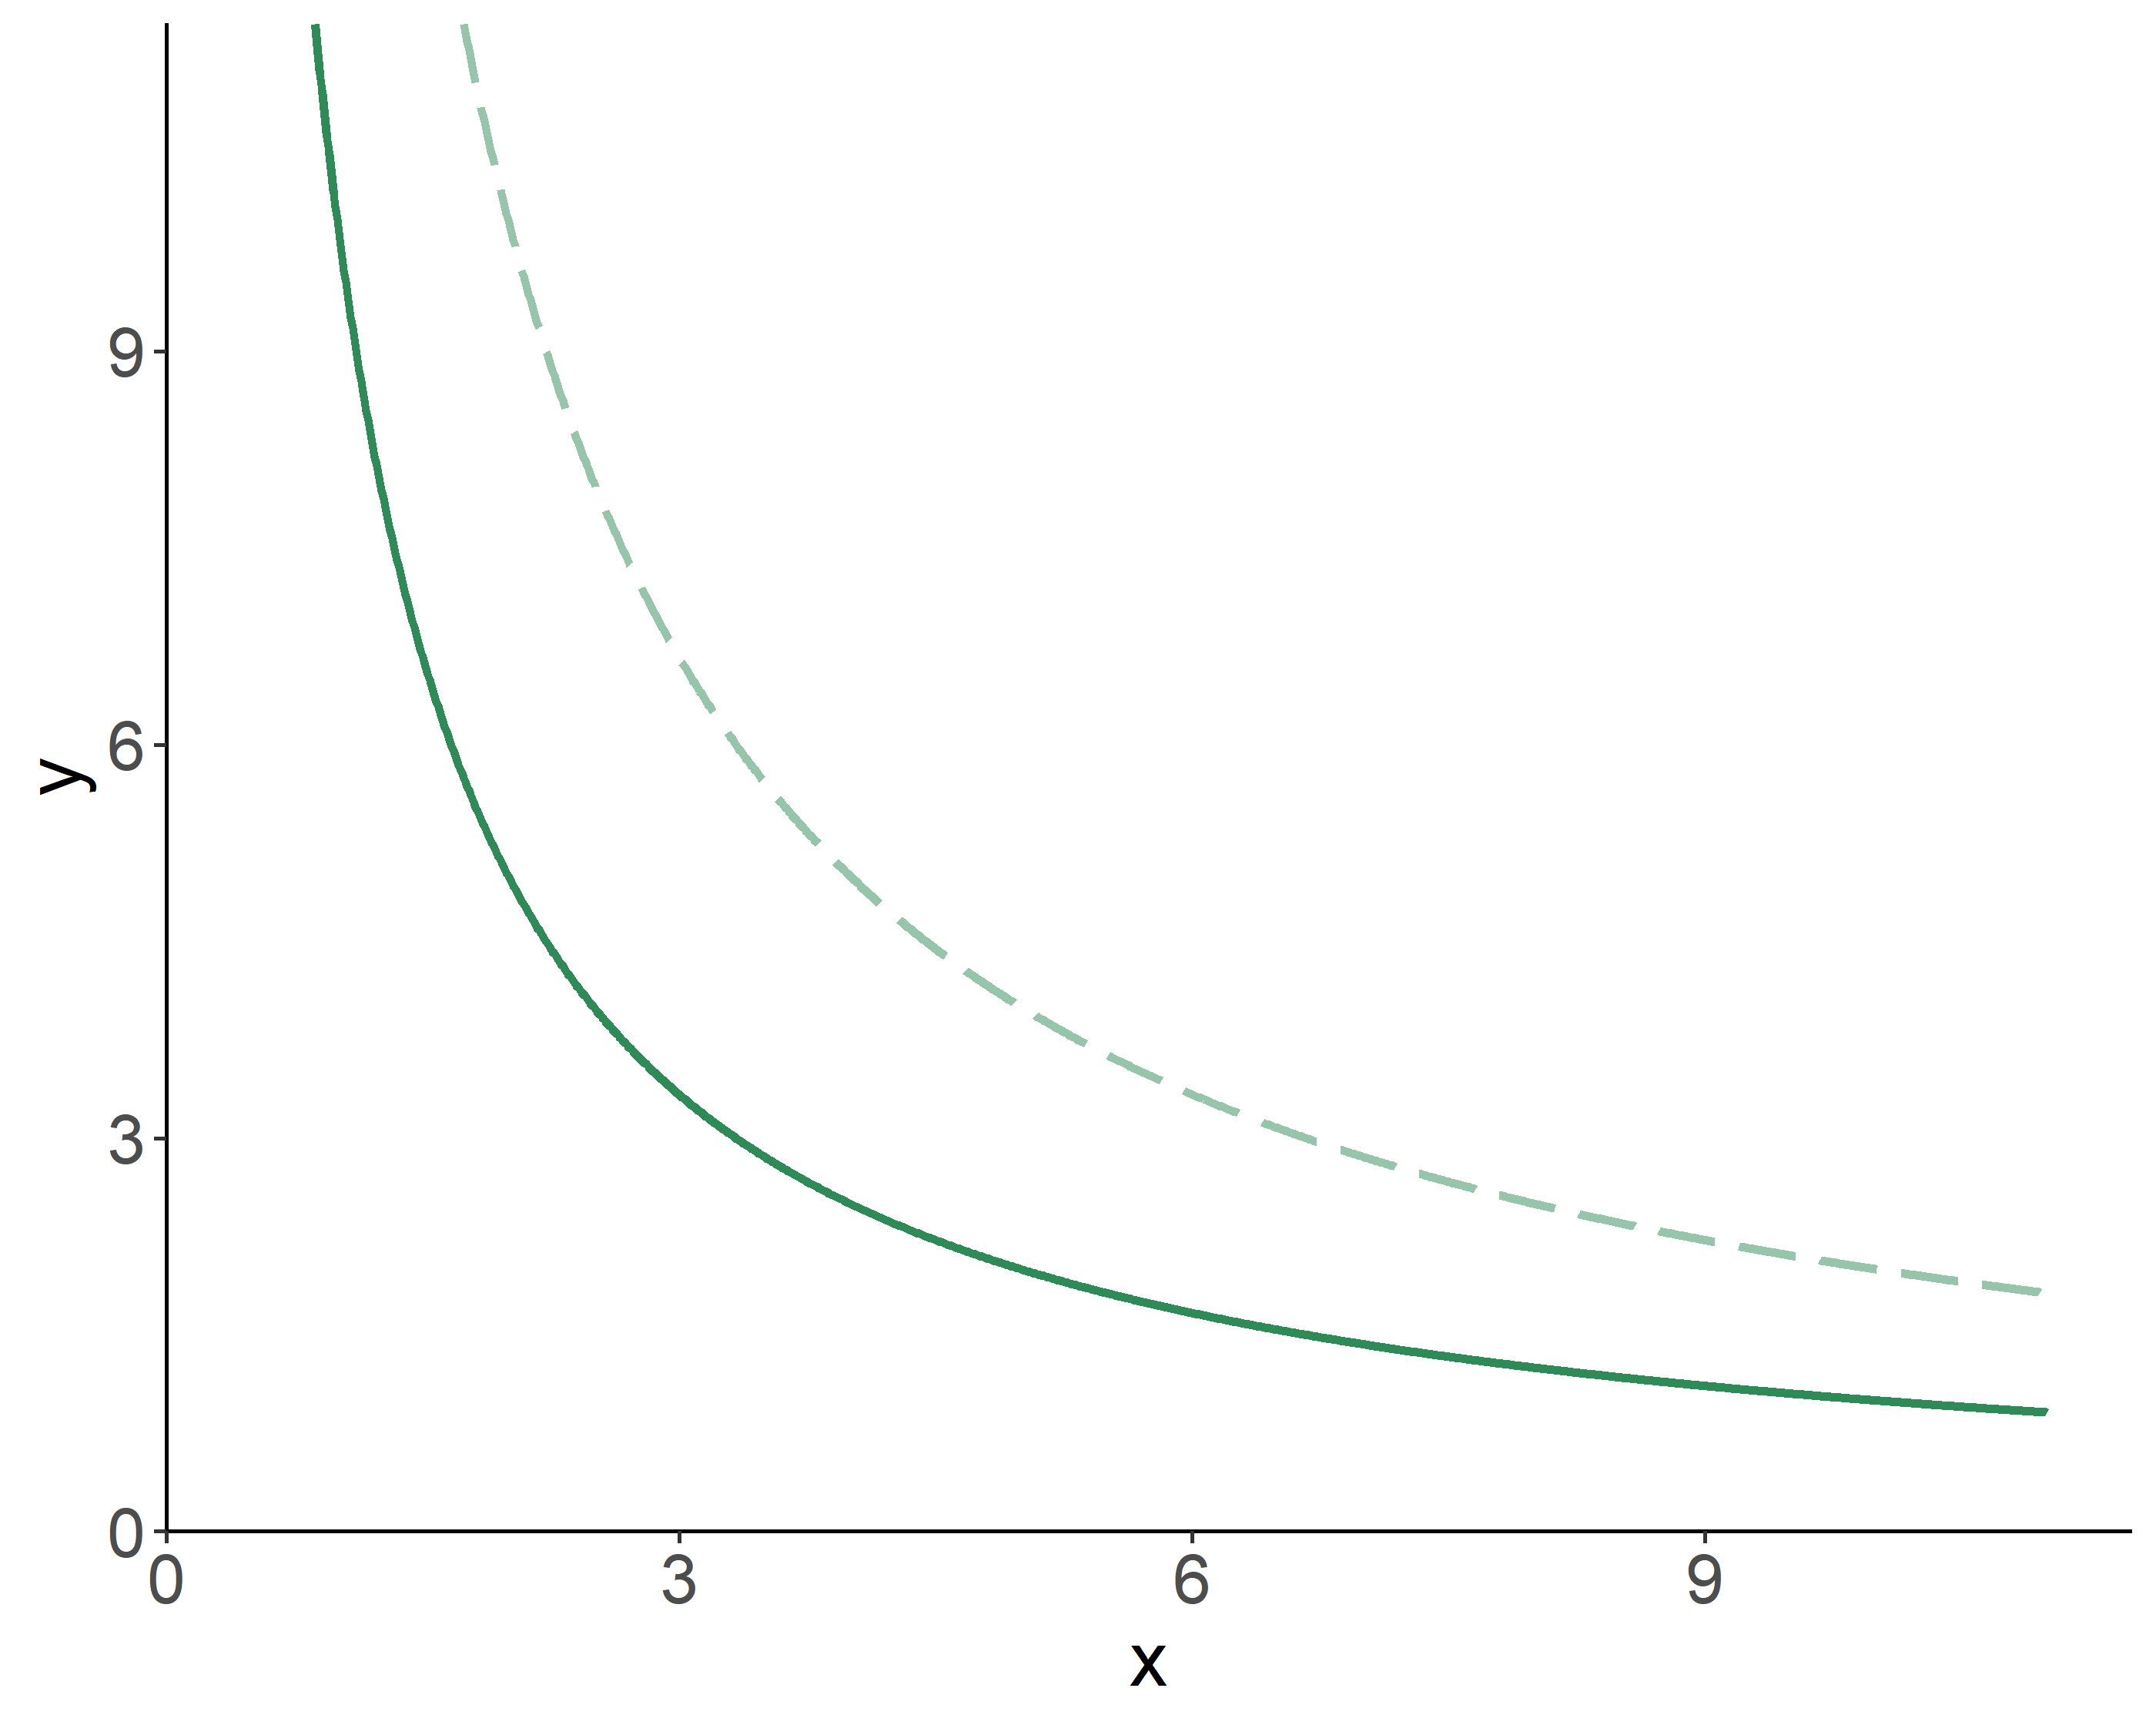
\includegraphics[width=0.9\linewidth]{envecon_files/figure-latex/ic-1} 

}

\caption{Indifference Curves}\label{fig:ic}
\end{figure}

Intuitively, because environmental pollution is a by-product of production of a market good, a consumer is left with a choice of giving up some of their desired good, to mitigate the damage to the environmental good. Note that different people (e.g., person \(i\) and person \(j\)) may choose to consume different amounts of the market good: \(x_i\neq x_j\); but everyone will consume the same amount of the environmental good: \(y_i=y_j=y\). Even so, the value, or the utility attained from this environmental good will vary among individuals.

There are many sources of utility from environmental goods (or negative utility from environmental bads):

\begin{itemize}
\tightlist
\item
  health benefits (e.g., lower incidence of respiratory problems);
\item
  productivity value (e.g., greenhouse gases increase temperature, which adversely impacts agricultural production);
\item
  use value (e.g., whale watching);
\item
  existence value (feeling good about clean environment);
\item
  altruism (feeling good knowing others enjoy clean environment)
\end{itemize}

Thus, the benefit provided to a person \(i\) by consuming the market and environmental goods is represented by a utility function: \(u_i(x_i,y)\).

\hypertarget{prices-and-the-optimal-choice}{%
\section{Prices and the Optimal Choice}\label{prices-and-the-optimal-choice}}

From an array of options, a person will choose an \emph{optimal bundle} of composite market and environmental goods, \(\left\{x^*,y^*\right\}\), such that their utility is maximized given their income, \(M\), and the prices of these two goods, \(p_x\) and \(p_y\). In other words, an individual's objective is to maximize the utility subject to the budget constraint.

\begin{figure}

{\centering 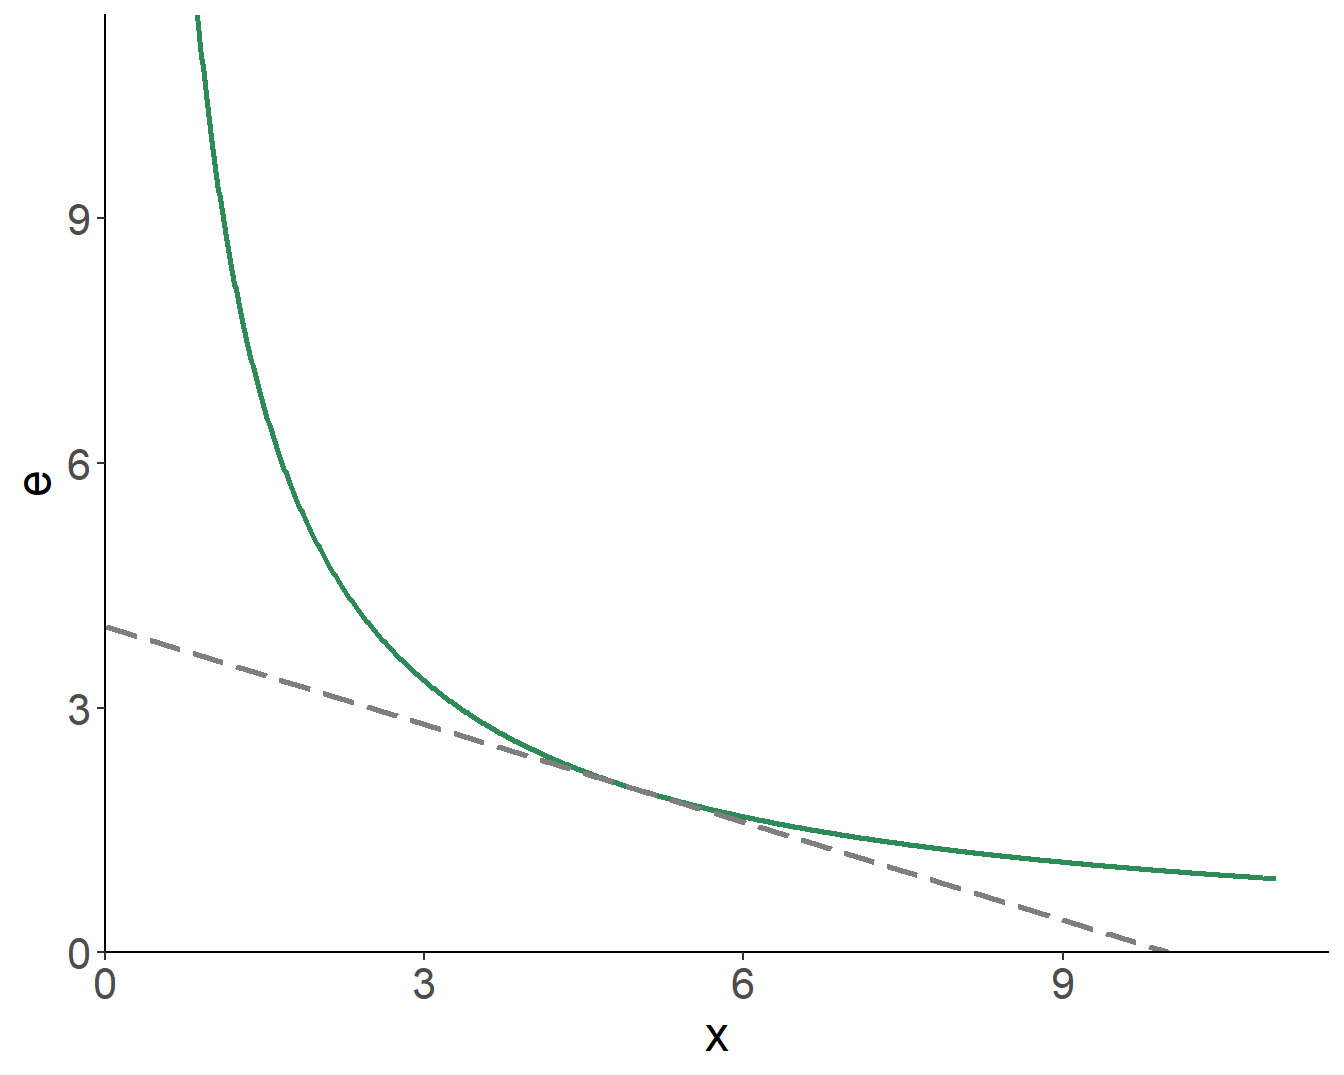
\includegraphics[width=0.9\linewidth]{envecon_files/figure-latex/optimal-1} 

}

\caption{Optimal Bundle}\label{fig:optimal}
\end{figure}

Mathematically: \[\max_{x,y}U(x,y),\;~~\mbox{s.t.}\;~p_{x}x+p_{y}y=M.\] The optimization leads to: \[\frac{MU_x}{MU_y} = \frac{p_x}{p_y}\] where the ratio of the two marginal utilities is referred to as the \emph{marginal rate of substitution}, \(MRS_{x,y}\), which indicates the amount of units of \(y\) a consumer is willing to give up to get a unit of \(x\).

\hypertarget{efficiency-in-exchange}{%
\section{Efficiency in Exchange}\label{efficiency-in-exchange}}

Consider achieving efficiency (in exchange of goods) in a two-person economy. In the illustrated \emph{Edgeworth Box}, any point on the plane represents an allocation of the two goods between the two individuals. The allocations along the contract curve---the dotted line on the graph---are Pareto optimal. For any given endowment (i.e., initial allocation), efficiency can be achieved along an array of points---the contract curve---where indifference curves of the two individuals are tangent to one another.

\begin{figure}

{\centering 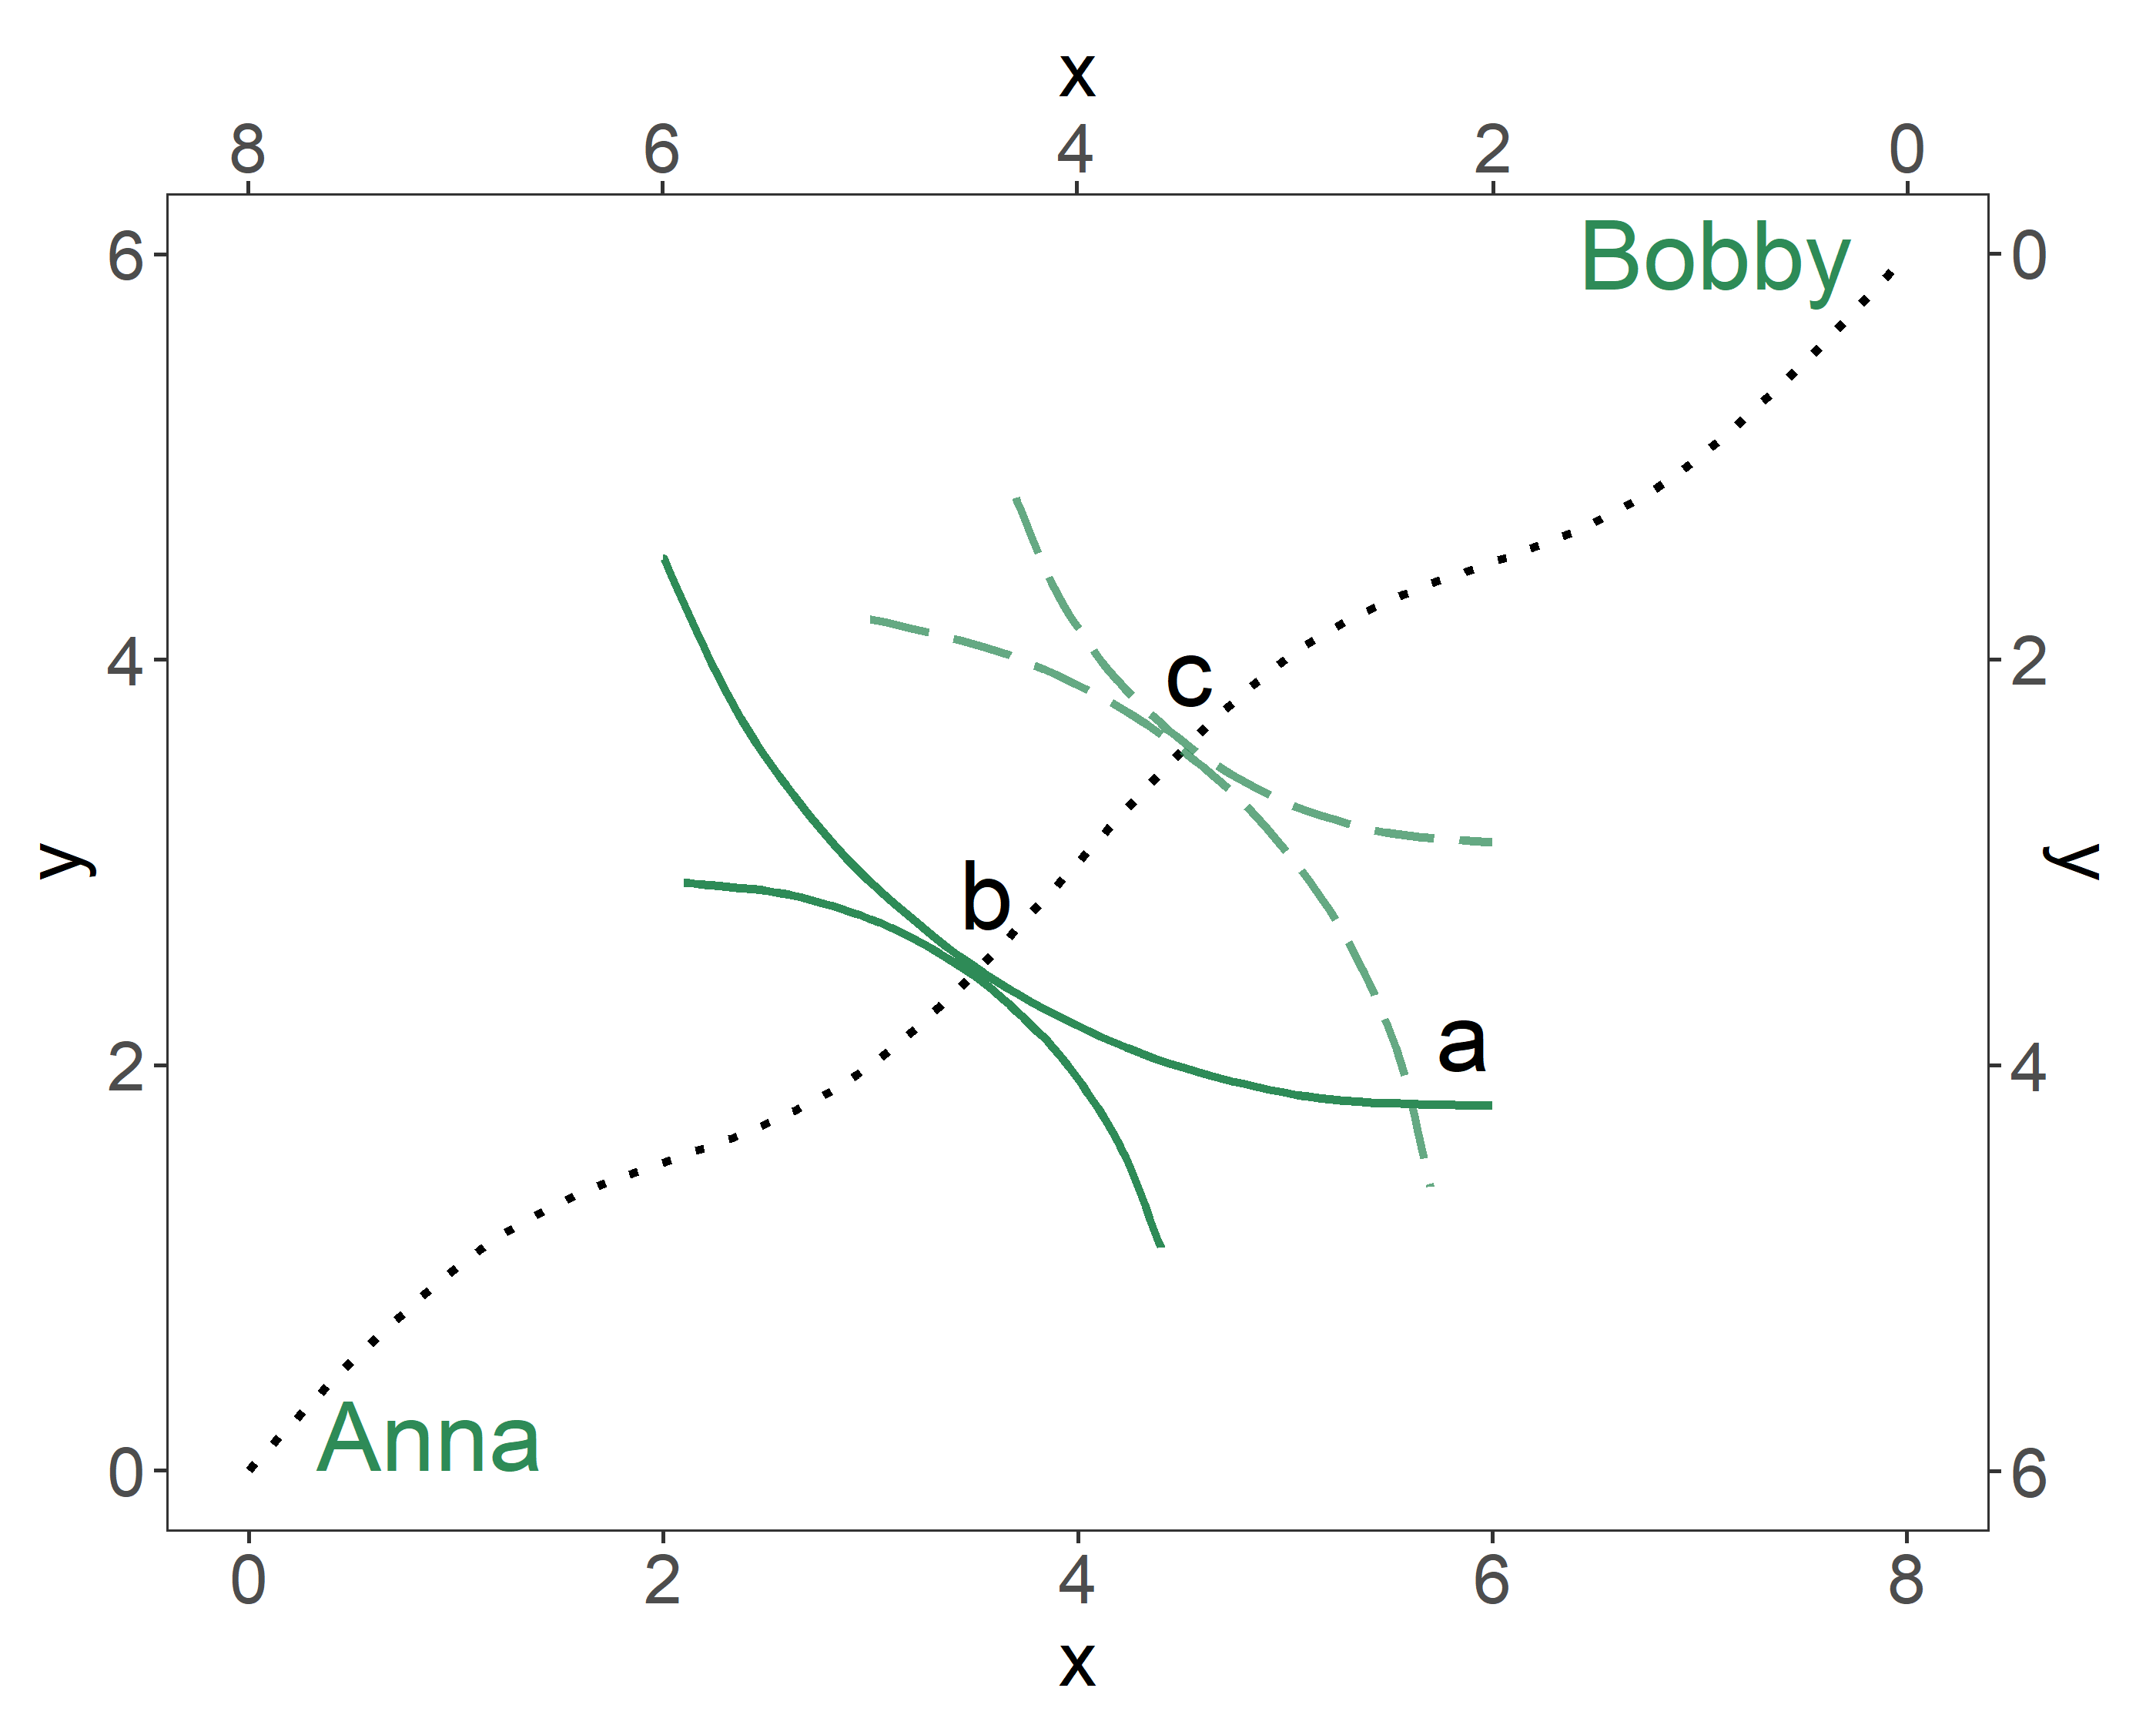
\includegraphics[width=0.9\linewidth]{envecon_files/figure-latex/edgeworth-1} 

}

\caption{Contract Curve}\label{fig:edgeworth}
\end{figure}

\hypertarget{social-choice-mechanisms}{%
\section{Social Choice Mechanisms}\label{social-choice-mechanisms}}

The foregoing discussion helps us understand (or, to some extent, conceptualize) an individual's preferences for a given bundle of market and environmental goods. But how about the society as a whole?

We can examine everyone's preferences, and if all happen to prefer some alternative over all other alternatives, we may conclude that the society as a whole prefers that alternative. This is also known as the \emph{Pareto criterion} for social choice.

Allocations on the \emph{Pareto frontier} are efficient, i.e., \emph{Pareto optimal}. Pareto optimality implies an allocation of goods at which it is impossible to make anyone better off, without making someone worse off. Pareto frontier is, in essence, the \emph{contract curve}.

An allocation is inefficient if it is interior to Pareto frontier. In such instance, a \emph{Pareto improvement} is possible. Pareto improvement implies an action that harms no one, and benefits at least one individual.

\begin{figure}

{\centering 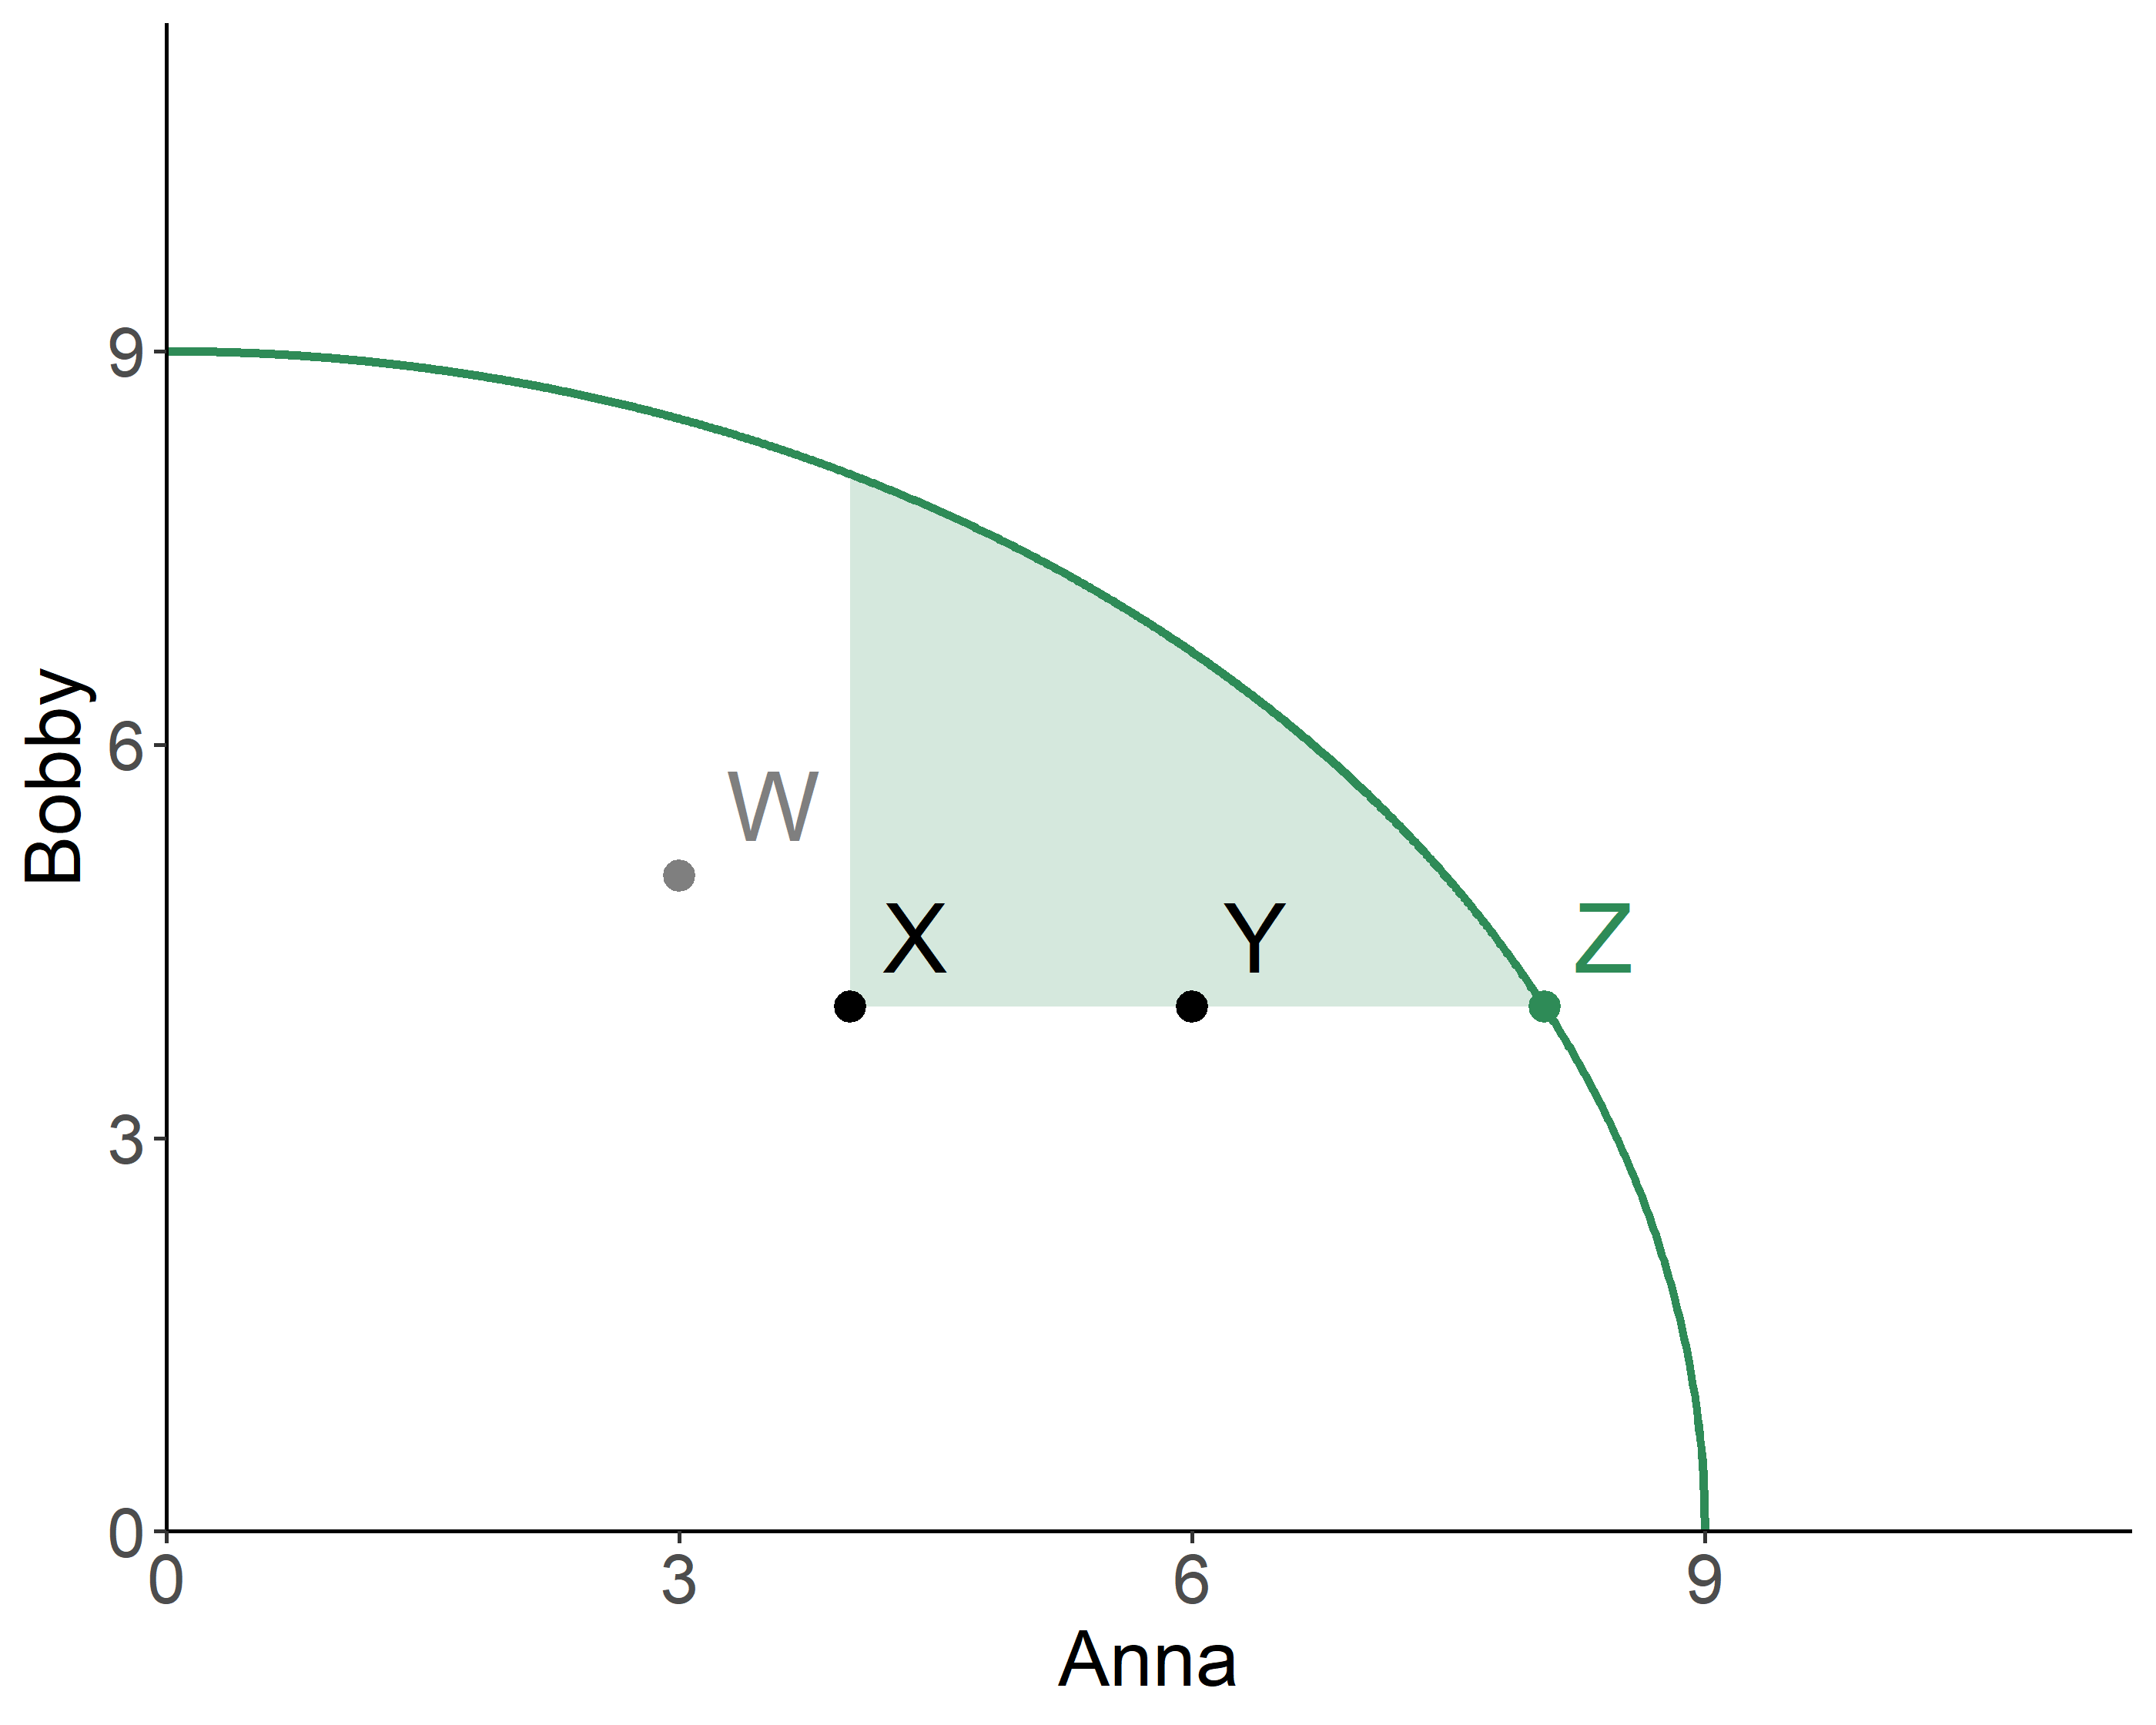
\includegraphics[width=0.9\linewidth]{envecon_files/figure-latex/pareto-1} 

}

\caption{Pareto Frontier}\label{fig:pareto}
\end{figure}

In the provided graph, the allocations \(X\), \(Y\), and \(Z\), are inefficient, and only the allocation \(Z\), is efficient. \(Y\), though inefficient, is Pareto improvement over \(X\). In fact, all allocations in the shaded region are Pareto improvements over \(X\).

The Pareto criterion is unanimity rule. For allocations \(a\) and \(b\), everyone must prefer the former to the latter for \(a\) to be Pareto preferred to \(b\). Because of this rule, decisions tend to be biased toward status quo, when Pareto criterion is applied to make societal decisions.

An alternative rule---that circumvents the issues associated with Pareto criterion---is \emph{unanimity with side payments}; that is, when member of society are allowed to transfer resources to increase the unanimity of opinion on alternative allocations. This approach, inherently, accounts for the extent to which individuals prefer one option to another. The rule leads to a \emph{potential Pareto improvement}, which implies an action that harms no one, and benefits at least one individual, after a set of net-zero transfers (side payments) have taken place.

Another mechanism---that relaxes the unanimity rule---is a voting mechanism based on the \emph{majority rule}. For allocations \(a\) and \(b\), if the majority prefers the former to the latter, we conclude that \(a\) is preferred to \(b\), even though there may be people in the society who strongly prefer \(b\) to \(a\).

\hypertarget{social-welfare-functions-and-impossibility-theorem}{%
\section{Social Welfare Functions and Impossibility Theorem}\label{social-welfare-functions-and-impossibility-theorem}}

A social welfare function is a way of representing societal preferences, akin to a utility function for individual preferences. If \(U_i(a)\) is the utility that a person \(i\) derives from choice \(a\), then \(a\) is said to be socially preferred to \(b\) if \(W[U_i(a):i=1,\ldots,N] > W[U_i(b):i=1,\ldots,N]\), where \(W[\cdot]\) is a social welfare function that summarizes the distribution of individual utilities in the society. Some of the well--known social welfare functions are:

\begin{itemize}
\tightlist
\item
  Utilitarian: \(W(U_i:i=1,\ldots,N) = \sum_i \theta_i U_i;\;~ \theta_i \ge 0, \sum_i\theta_i=1\)
\item
  Egalitarian: \(W(U_i:i=1,\ldots,N) = \sum_i U_i-\lambda\sum_i[U_i-\min(U_i)]\)
\item
  Rawlsian: \(W(U_i:i=1,\ldots,N) = \min(U_i)\)
\end{itemize}

For a social choice mechanism to work, it should satisfy the following assumptions:

\begin{itemize}
\tightlist
\item
  Completeness---we should be able to compare alternatives.
\item
  Unanimity---if everyone in the society prefers \(a\) to \(b\), then the society should prefer \(a\) to \(b\).
\item
  Nondictatorship---no one's preferences should be exactly the same as those of the society.
\item
  Universality---any possible individual rankings of alternatives is allowed.
\item
  Transitivity---if \(a\) is socially preferred to \(b\), and if \(b\) is socially preferred to \(c\), then \(a\) should be socially preferred to \(c\).
\item
  Independence of Irrelevant Alternatives---social preference between two alternates should only depend on people's preferences for these two, regardless of their preferences for any other alternatives.
\end{itemize}

These are the axioms put forward by Kenneth Arrow. In what became to be known as \emph{Arrow's Impossibility Theorem} he proved that there is no rule satisfying all six assumptions that can convert individual preferences into a social preference ordering.

\hypertarget{market-failure}{%
\chapter{Market Failure}\label{market-failure}}

Kolstad (\protect\hyperlink{ref-kolstad2010}{2010}, Chapter 5); Keohane and Olmstead (\protect\hyperlink{ref-keohane2016}{2016}, Chapter 5)

In a competitive market, the interaction of market demand and supply curves results in the equilibrium price and quantity that are Pareto optimal (the first theorem of welfare economics). That is, no other price--quantity combination can yield a larger total surplus than that presented by the competitive equilibrium. Moreover, in a competitive market, a Pareto optimal equilibrium can be achieved, provided that initial endowments are appropriately distributed (the second theorem of welfare economics).

The competitive equilibrium does not always yield the socially optimal price--quantity combination, however. The reasons for this could be linked with concepts known as \emph{externality}, \emph{common property}, and \emph{public goods}.

\hypertarget{externality}{%
\section{Externality}\label{externality}}

In unregulated markets, firms' costs typically do not account for the environmental damages (e.g., pollution)---usually associated with the production process---the supply is shifted outward compared to the socially optimal supply. That the market supply is not the same as the socially optimal supply is because of externalities. Externality is an effect of an action of one party on the utility or production function of another party without that party's permission or compensation.

Consider two firms that are located near a river: a steel factory (upstream), which dumps the waste into the river, and a resort (downstream), which uses river for recreation. In absence of externality, the outputs of these two firms (\(y^u\) and \(y^d\)) are independent of each other. With externality, which is the waste from the steel factory, \(y^d\) can be seen as a decreasing function of \(y^u\). A production externality exists when profits of one firm are (involuntarily) affected by those of another.

\begin{figure}

{\centering 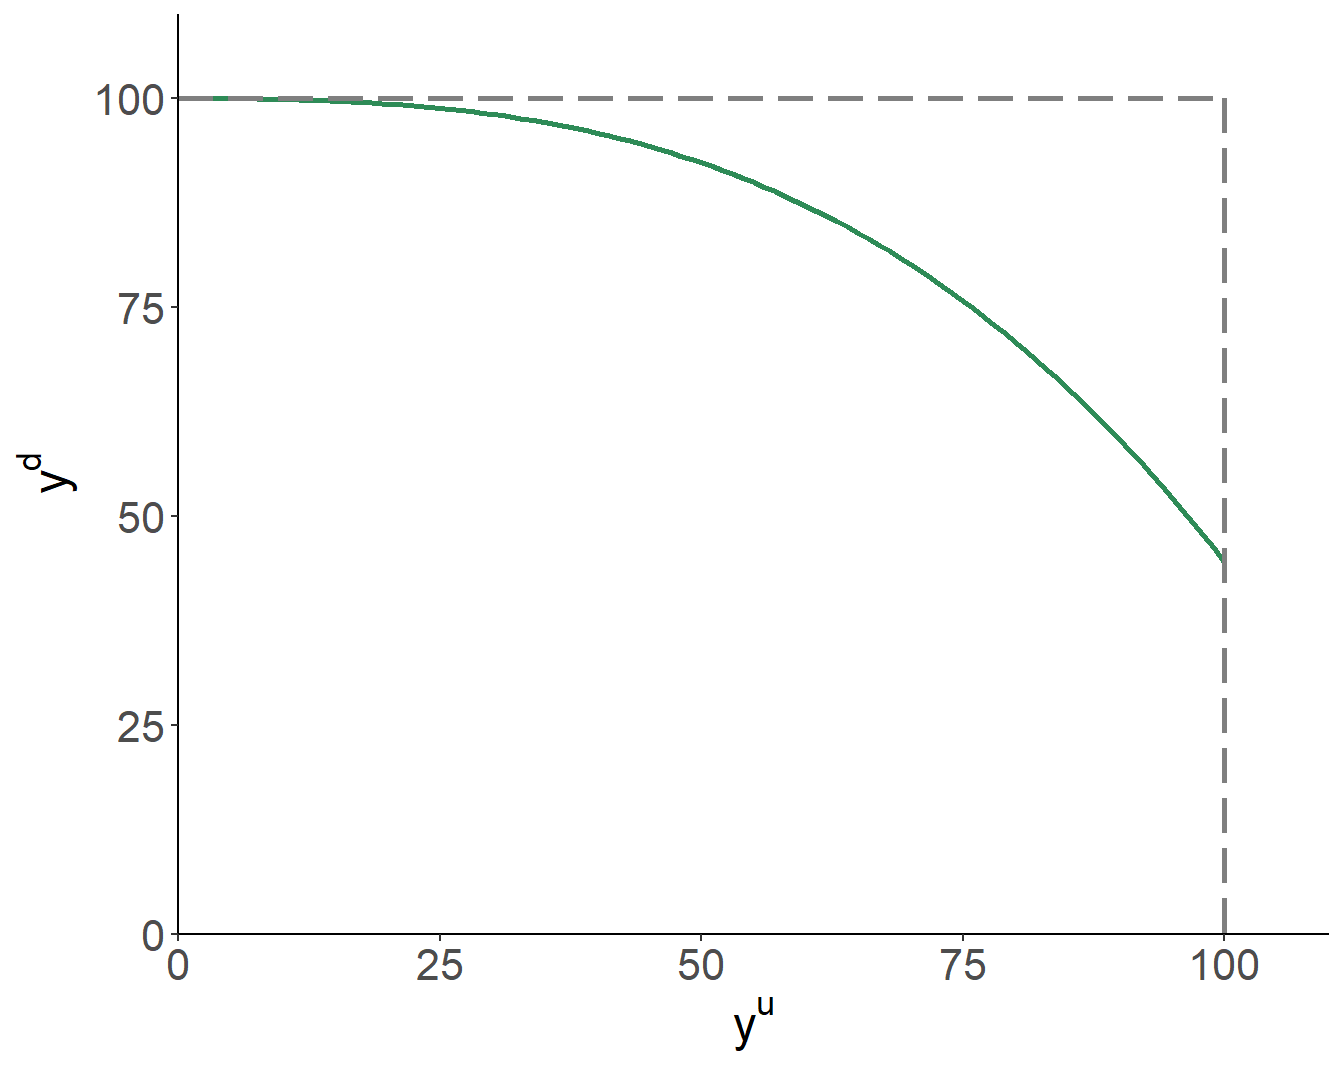
\includegraphics[width=0.9\linewidth]{envecon_files/figure-latex/production-1} 

}

\caption{Production Externality}\label{fig:production}
\end{figure}

A way to resolve the issue of the externality is to make it part of the producer's cost function. Recall that the efficient quantity of production/consumption is the quantity at which demand (which is, indeed, marginal benefit) is equal to supply (i.e., marginal cost). This equilibrium accounts for consumers and producers, but the society also includes a `third party.' Thus, we need to make a distinction between the marginal cost (of production), \(MC\), the marginal external cost, \(MC^e\); and the sum of the two, which is the marginal social cost, \(MC^s = MC+MC^e\).

The marginal external cost can be negative or positive. For negative externalities (e.g., pollution, noise), \(MC^s > MC\) (or, equivalently, \(MC^e > 0\)). The market, on its own, has a tendency to produce \(Q^c>Q^s\); that is, the market tends to lead to overproduction. In the previous example, this would be the overproduction of steel by the factory.

\begin{figure}

{\centering 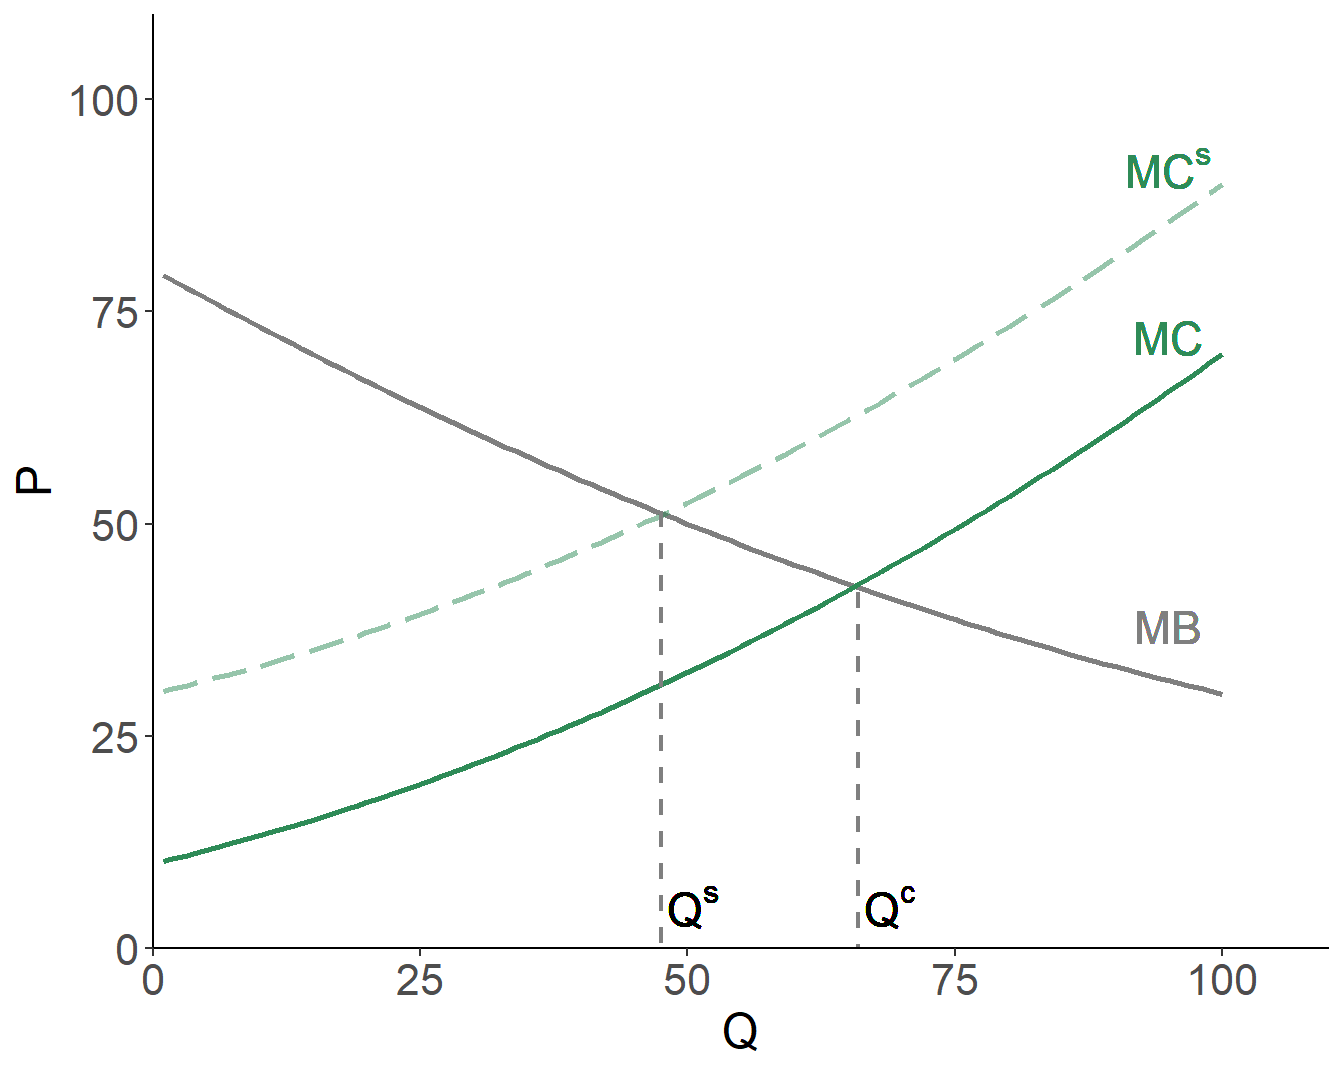
\includegraphics[width=0.8\linewidth]{envecon_files/figure-latex/externality-1} 

}

\caption{Negative Externality}\label{fig:externality}
\end{figure}

For goods that offer positive externality, such as vaccinations, blog-posts, well-maintained front-yards, \(MC^s < MC\) (or, equivalently, \(MC^e < 0\)). The market, thus, has a tendency to produce (and consume) too little compared to the socially optimal outcome (\(Q^c < Q^s\)). In other words, when left unregulated, the market tends to lead to underproduction.

\hypertarget{common-property}{%
\section{Common Property}\label{common-property}}

Another reason as to why markets fail with environmental goods is that most environmental goods are \emph{open access}, or \emph{common property}, which leads to the potential overuse of these goods---a phenomenon referred to as the \emph{tragedy of commons}. People overuse common property because they do not bear the full costs of their actions (i.e., the costs of their actions on others). For example, highways that tend to be highly congested during the rush hours; or pollution from factories that treat the airshed as everyone's property for waste disposal.

In all instances, when one person consumes the good, the marginal cost to others of consuming that good increases. To illustrate the point, consider the case of a fishery. The fish are valuable, but it takes effort to catch them. The effort is inversely proportional to the number (or density) of fish in the water. A person will engage in fishing as long as it is profitable.

\begin{figure}

{\centering 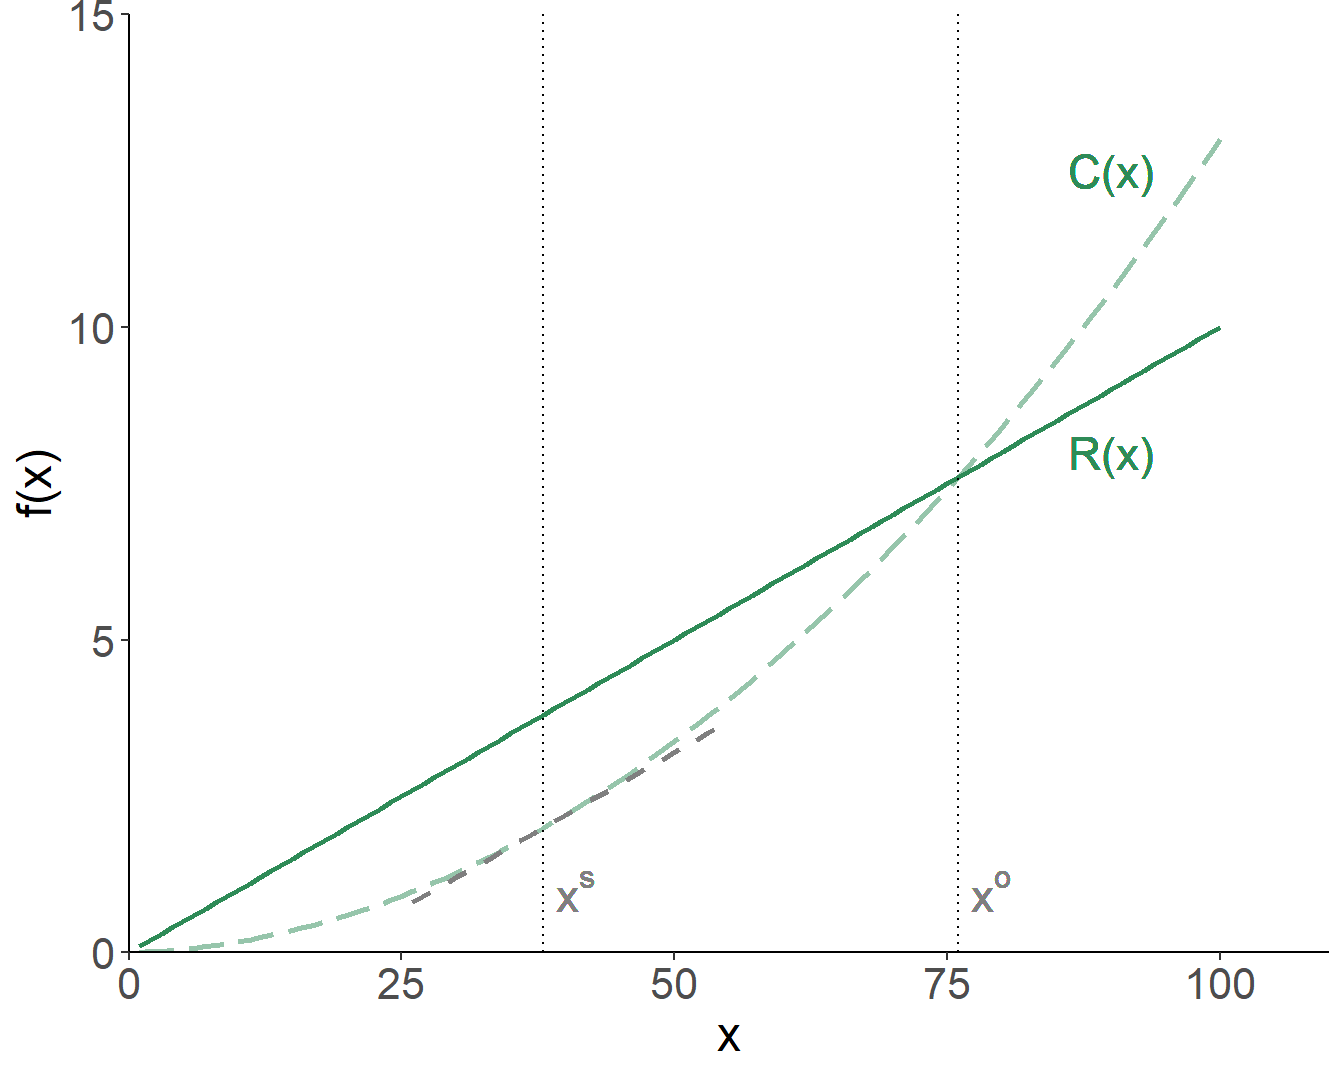
\includegraphics[width=0.8\linewidth]{envecon_files/figure-latex/common-1} 

}

\caption{The Overuse of Common Property}\label{fig:common}
\end{figure}

In this illustration, profits are exhausted at \(x^o\), even though the socially efficient amount of output is \(x^s\). The problem exists because fishermen only take into the account their individual marginal costs in their decision-making. Because people do not account for the costs of their actions on others, the common property is overused.

\hypertarget{public-goods-and-bads}{%
\section{Public Goods (and Bads)}\label{public-goods-and-bads}}

The important characteristic about a public good is that, once provided, many people jointly share in its benefits (e.g., clean air, highway, national defense). Public goods are not necessarily provided by the government, but they often are (and for good reason).

Two important characteristics of a public good (or bad) are \emph{excludability} and \emph{rivalry}.

Excludability has to do with whether it is possible to use prices to ration individual use of the good. A good is excludable if it is feasible (and practical) to selectively allow individuals to consume the good.

To be able to use prices to allocate goods, it must be possible to keep individuals from the goods, unless they have paid an appropriate price. Two factors play role in excludability: (i) the cost of exclusion, and (ii) the technology (and its evolution over time) of exclusion. Excludability enables a price system to work.

Rivalry has to do with whether it is desirable to ration individual use of the good, through prices or any other means. A good is rival if one person's use of the good, diminishes or prevents the use of that good by others.

Based on degrees of excludability and rivalry, goods can be classified into four broad categories:

\begin{longtable}[]{@{}lll@{}}
\toprule
& \textbf{Rival} & \textbf{Non-Rival}\tabularnewline
\midrule
\endhead
\textbf{Excludable} & private goods & club goods\tabularnewline
\textbf{Non-excludable} & common property & public goods\tabularnewline
\bottomrule
\end{longtable}

To obtain aggregate demand, with private goods (or rival goods, more generally) we add up the demand curves horizontally, with public goods (or non-rival goods, more generally) we add up the demand curves vertically. Therefore, we cannot infer the market price for non-rival goods from the intersection of aggregate demand and supply curves---as we do so for rival goods---as the individual demands will end up being too low.

\hypertarget{environmental-valuation}{%
\chapter{Environmental Valuation}\label{environmental-valuation}}

Kolstad (\protect\hyperlink{ref-kolstad2010}{2010}, Chapters 7 \& 10); Adamowicz et al. (\protect\hyperlink{ref-adamowicz1998}{1998})

Actions of firms---which are directed to maximize their profits, and often result in environmental pollution of some sort---are primarily motivated by consumer demand for goods offered by these firms. The demand functions tells us:

\begin{itemize}
\tightlist
\item
  how much a person will spend on a given good out of an array of options;
\item
  the marginal valuation a consumer places on a good at different consumption levels; and
\item
  how much of the good an individual is willing to forgo if the price increases.
\end{itemize}

Things are different with environmental goods, because there are no markets for those. For example, for an environmental good such as `clean air,' we do not have information on different consumption levels at different prices, even though people who value clean air more would be willing to pay a higher price for an `additional unit' of the air quality.

\hypertarget{willingness-to-pay}{%
\section{Willingness to Pay}\label{willingness-to-pay}}

Valuation (of a good) is an individual--specific measure that depicts the maximum amount of money a person would be willing to give up to obtain a unit amount of the good. For example, willingness to pay (WTP) for the environmental good (e.g., certain degree of air quality) is the dollar amount an individual is willing to give up, to obtain such air quality. WTP is the amount which, if paid in exchange for a good or service, leaves a person just as well off as without paying and without receiving the good or service. The concept of the WTP for environmental quality is closely linked with the concept of damages due to the reduction of environmental quality.

\hypertarget{measuring-demand-for-environmental-goods}{%
\section{Measuring Demand for Environmental Goods}\label{measuring-demand-for-environmental-goods}}

Two basic approaches to measuring demand rely on \emph{revealed preferences} and \emph{stated preferences}. In revealed preference, the actual choices are observed, which allows us to infer the values of environmental goods. The usual `problem' with this approach is that, it is not directly applicable to goods for which markets do not exist (e.g., most environmental goods).

In stated preference, the actual choice is not observed, rather people are asked to report (state) how they would trade-off money for the good if they were to face such a choice. Thus, the stated preference method allows us to directly examine individuals' valuation for goods and services for which markets do not exit. The issue with this approach is with the hypothetical nature of information---when asked, people may understate or overstate their valuation for some strategic reasons or simply due to the carelessness.

\hypertarget{revealed-preferences}{%
\section{Revealed Preferences}\label{revealed-preferences}}

Even though markets rarely exist for environmental goods, the observed demand for market goods in different `environmental scenarios' may help us with the valuation of environmental goods.

\hypertarget{hedonic-method}{%
\subsection{Hedonic Method}\label{hedonic-method}}

Consider housing as an example of a market good, \(x\), and air quality as an environmental good, \(e\). Let \(p_x\) denote the housing price. The goal is to infer the value of the environmental good. The relationship between the housing prices, air quality and quantity of housing demanded can be given by: \(x=h(p_x,e)\); that is, the demand for housing is a function of its price, as well as the air quality in the neighborhood. Turns out, such demand function can help us understand the demand for the environmental good, which is equivalent to marginal WTP of \(e\).

\begin{figure}

{\centering 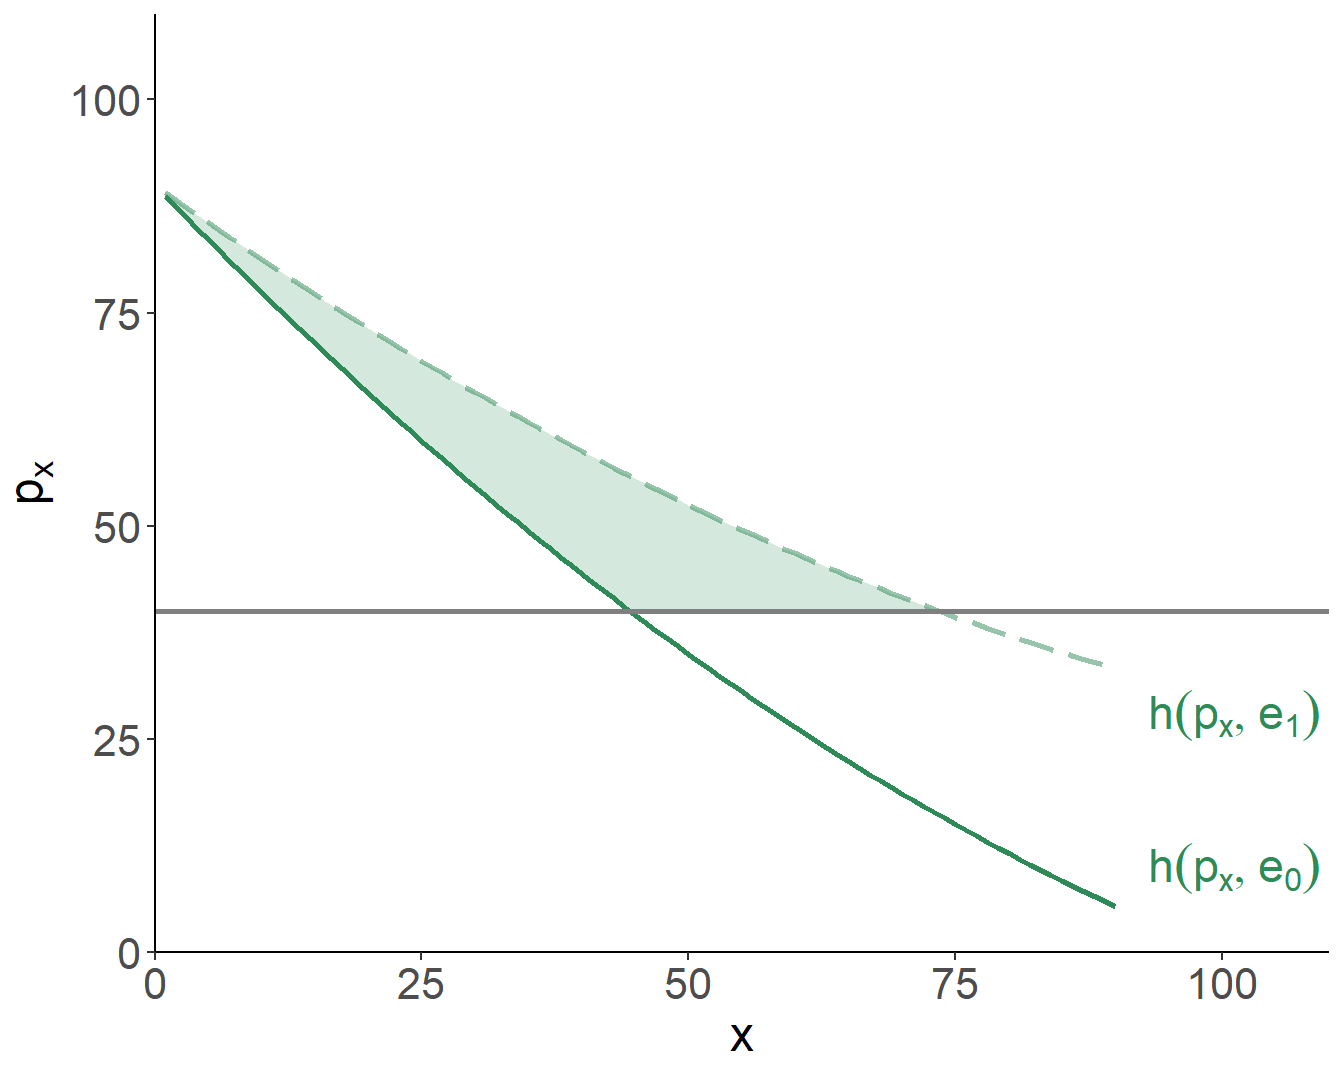
\includegraphics[width=0.8\linewidth]{envecon_files/figure-latex/wtp-1} 

}

\caption{WTP for Clean Air}\label{fig:wtp}
\end{figure}

If the only purpose of the air quality were to enhance the experience of consuming the market good in consideration, the foregoing analysis addresses the question of obtaining demand for an environmental good. But air quality surely affects individuals' well-being in ways unrelated to housing. So, the `estimated' value of the environmental good is, really, a lower bound---only a portion of total value attached to the air quality is captured. An additional challenge, in such analysis, is accounting for all other factors that affect housing demand.

\hypertarget{travel-cost-method}{%
\subsection{Travel Cost Method}\label{travel-cost-method}}

Travel cost method infers values of environmental goods by examining costs that visitors incur getting to a recreational site and then using this information to estimate willingness to pay that site.

As another example, consider a range of recreational sites located at some distance from a city. People travel to these sites with different levels of environmental amenities. When they do so, they incur different costs (costs of transportation; membership/entrance fees; opportunity costs of time). Thus, people's demand for environmental good (available at these recreational sites) can be inferred from costs they incur in the process.

\hypertarget{stated-preferences}{%
\section{Stated Preferences}\label{stated-preferences}}

Demand for a range of environmental goods may not be examined using (previously discussed) revealed preference methods. Existence value, for example, is very difficult (if not impossible) to estimate based on actual behavior of individuals, because their choices with regard to market goods are unaffected by whether or not `that something' is available. Moreover, for many environmental goods, there is no market for ordinary goods, through which their value can be reflected. This has motivated researchers to develop valuation techniques that involve the construction of a market, when such market is absent.

Two broad categories of constructed markets exist: hypothetical and experimental. Valuation though hypothetical constructed markets is referred to as stated preference, or \emph{contingent valuation}. In such hypothetical scenarios, potential consumers are asked to state their valuation of a good, if there were a market for such good (hence the term `contingent').

In the case of the experimental constructed markets, a researcher constructs all the (desired) characteristics of a market, and then observes participant's behavior within this market. In the case of \emph{choice experiment}, for example, a researcher presents a respondent with a choice of scenarios, with a price tag attached to each scenario, and a respondent chooses the preferred option; the choice set typically includes the the \emph{status quo} (i.e., the `no change') option as well.

\hypertarget{wtp-vs-wta}{%
\section{WTP vs WTA}\label{wtp-vs-wta}}

Thus far we have focused on WTP---the dollar amount someone would be willing to give up to obtain something. Another related and relevant measure is willingness to accept (WTA)---the dollar amount someone would be willing to accept in compensation for giving up something.
Conceptually, WTP and WTA seem to be `mirror images' of some sort: how much will an individual pay to live in a neighborhood with less air pollution vs.~how much of a compensation will an individual accept to live in a neighborhood with more air pollution. Theoretically (as well as in practice), these two measures are not necessarily identical, however.

Consider an environmental good, \(e\), and a market good, \(x\). Let a starting bundle be \(\{x_0,e_0\}\), yielding utility: \(U_0 = U(x_0,e_0)\). Consider also an alternative bundle, \(\{x_0,e_1\}\), yielding utility: \(U_1 = U(x_0,e_1)\). We are interested in two measures:

\begin{itemize}
\tightlist
\item
  starting at \(e_0\), the WTP to move to \(e_1\); and
\item
  starting at \(e_1\), the WTA to move to \(e_0\).
\end{itemize}

\begin{figure}

{\centering 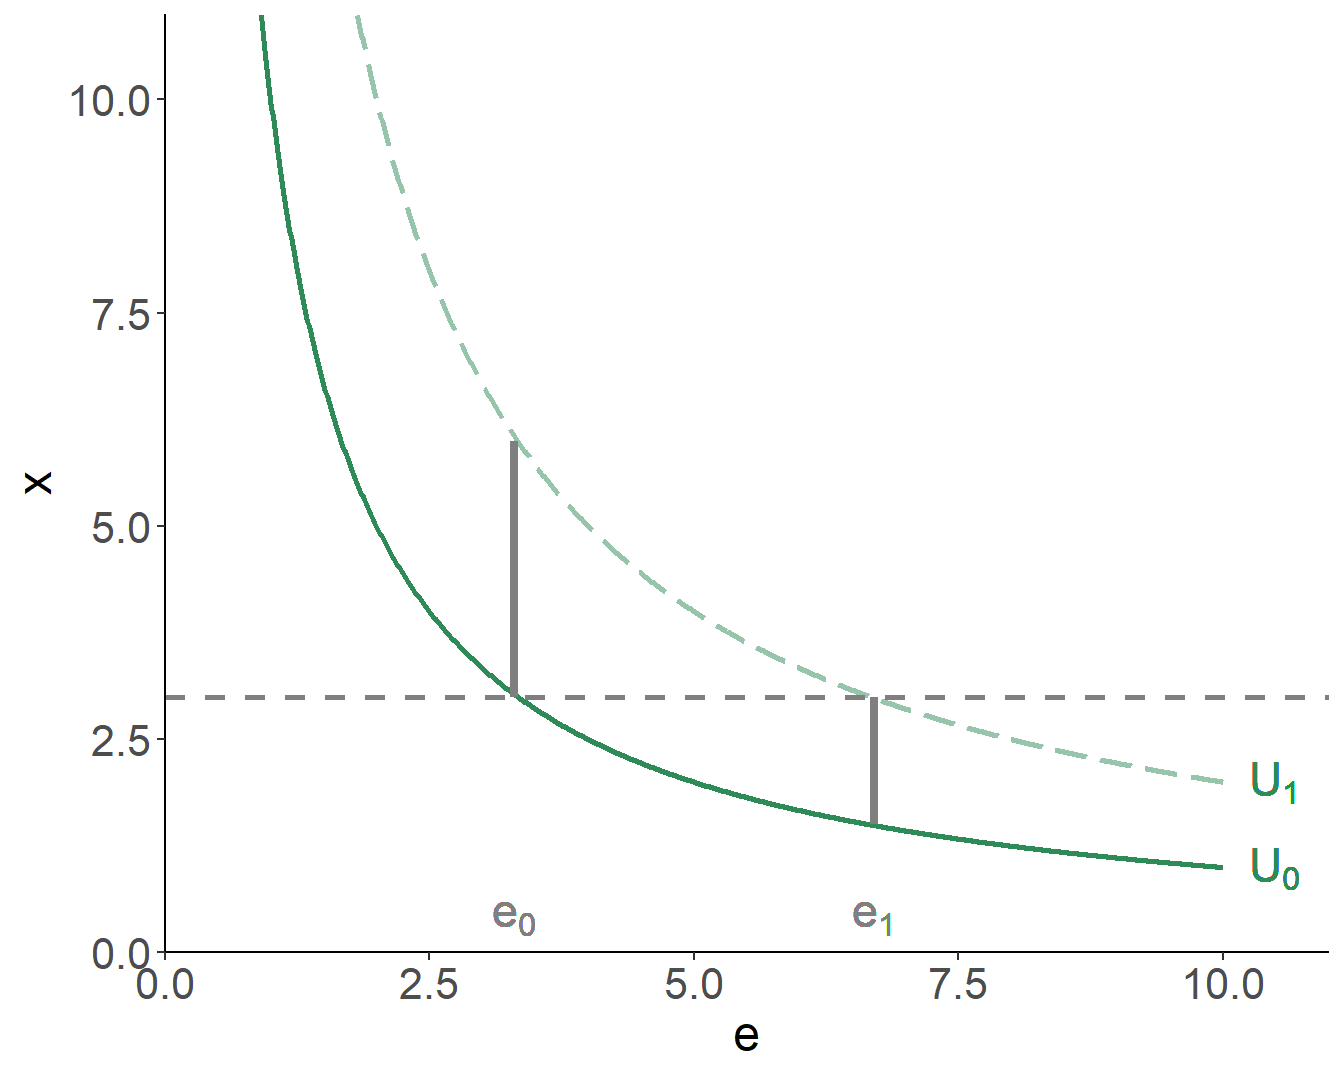
\includegraphics[width=0.8\linewidth]{envecon_files/figure-latex/valuation-1} 

}

\caption{WTP vs WTA}\label{fig:valuation}
\end{figure}

As seen, WTA \(>\) WTP, which is the result of the indifference curves being convex to the origin, implying that as an individual decreases consumption of an environmental good, larger amounts of the market good are required to keep utility unchanged. This result is driven by the substantial change in the environmental good, otherwise---within a smaller region of the graph---indifference curves would be nearly linear, resulting in approximately equal WTP and WTA measures.

\hypertarget{property-rights}{%
\chapter{Property Rights}\label{property-rights}}

Kolstad (\protect\hyperlink{ref-kolstad2010}{2010}, Chapter 13); Isaksen and Richter (\protect\hyperlink{ref-isaksen2019}{2019})

With environmental goods, \emph{non-excludability} is one of the main causes of market failure. One way to tackle the issue is by establishing \emph{property rights}. This simple institutional intervention makes goods excludable, and allows markets to operate efficiently. For this to work, property rights should be \emph{well-defined}, \emph{transferable}, \emph{secure}, and \emph{complete}.

\hypertarget{coase-and-the-assignment-of-rights}{%
\section{Coase and the Assignment of Rights}\label{coase-and-the-assignment-of-rights}}

Who should be assigned rights: the party creating the externality (the `culprit') or the party affected by the externality (the `victim')? Ronald Coase raised this issue, back in 1960. Consider a case of air pollution. The problem with air pollution arises because a culprit happens to be located too close to victims. But one may also argue that a polluter is only a culprit because people who breathe polluted air happen to live too close to the polluter. So, should it be a culprit who is given the right to pollute, or should it be victims who are assigned the right to breathe clean air? Coase's conclusion was that because the right to pollute and the right to breathe clean air are property rights that have value, as long as trade is allowed, efficiency should prevail, no matter how those rights are initially distributed.

As an example, consider two firms: a steel manufacturer, which dumps the waste into the river, and a resort, which needs clean river for proper functionality. Let the firms' profits be given by: \(\pi_s(a)\) and \(\pi_r(a)\), where \(a\) is the level of abatement which can go from 0 (no abatement) to 1 (full abatement and no pollution). The optimal level of abatement, \(a^*\), is where the marginal benefit of abatement equals the marginal costs of abatement.

\begin{figure}

{\centering 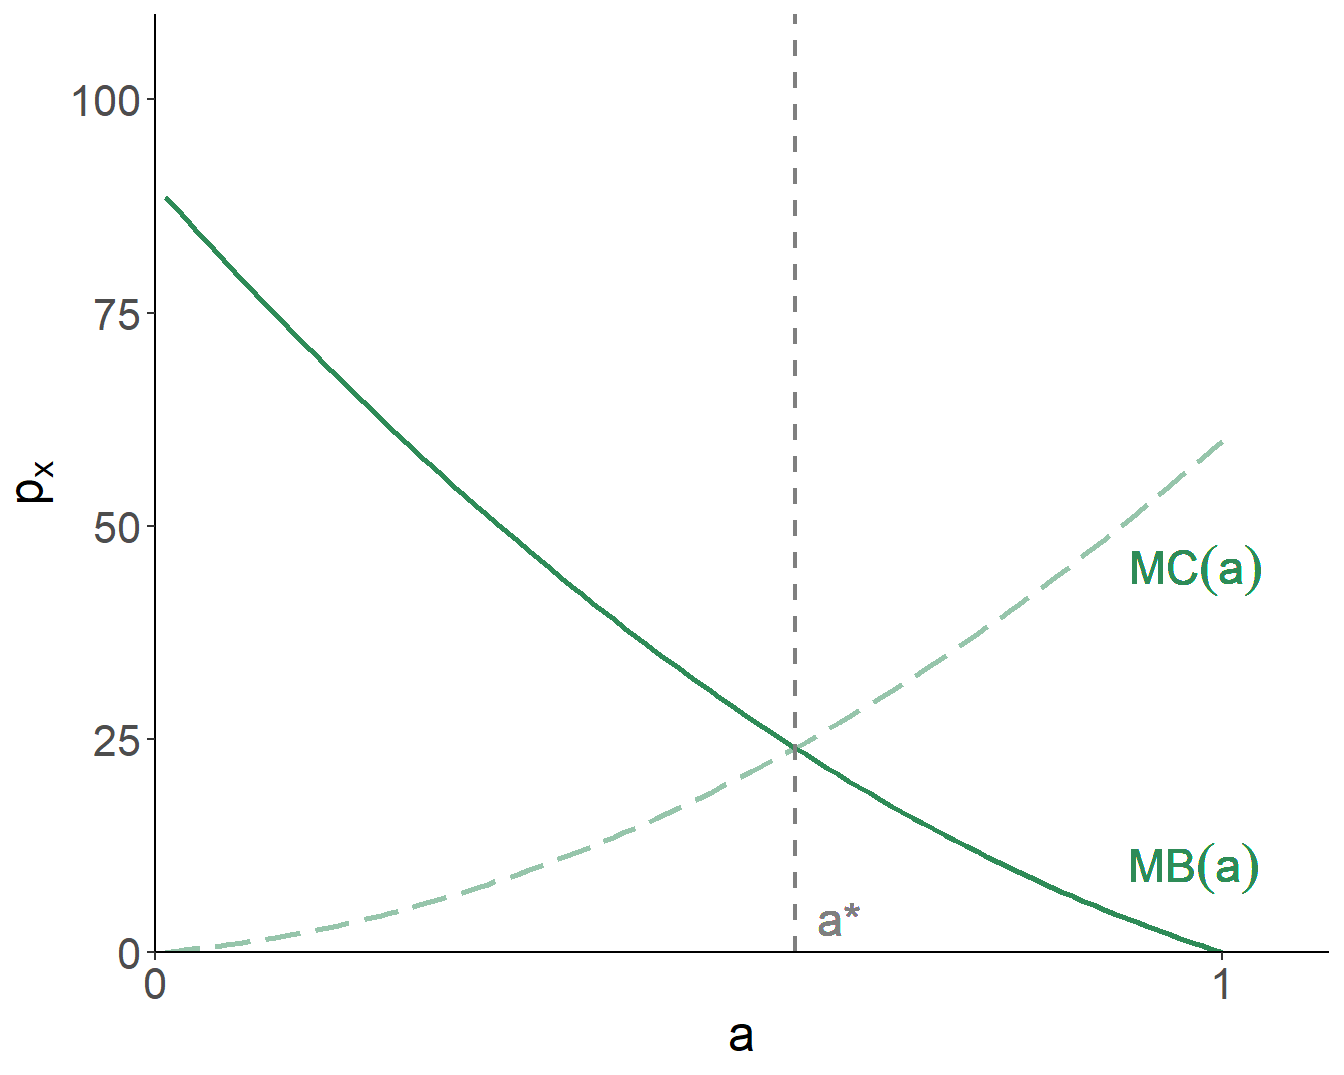
\includegraphics[width=0.8\linewidth]{envecon_files/figure-latex/abatement-1} 

}

\caption{Optimal Abatement}\label{fig:abatement}
\end{figure}

At this level, the cumulative profit is: \(\pi_s(a^*)+\pi_r(a^*)\). There are two other possible outcomes, where either one of the two facilities cease to operate. In those instances, the cumulative profit will simply be the profit of one or the other businesses---i.e., \(\pi_s(0)\) or \(\pi_r(1)\)---that has remained open. From the efficiency standpoint, the largest total profit level dictates the action to be taken.

\hypertarget{the-victim-has-rights}{%
\subsection{The Victim Has Rights}\label{the-victim-has-rights}}

Suppose the resort has the legal right to clean water; that is, the right to complete abatement, \(a=1\). In this scenario, the profits of the two firms are: \(\pi_s(1)\) and \(\pi_r(1)\). If the steel manufacturer wants to pollute (produce, that is), it will have to compensate the resort for any damage. That is, the resort's profit is guaranteed to be at least \(\pi_r(1)\). At \(a=1\) the marginal cost of abatement exceeds the marginal benefit, so there is room for negotiation to reduce the abatement level.

In fact, the abatement will end up at \(a^*\), where the marginal cost of abatement equals the marginal benefit. The steel manufacturer has the following options:

\begin{itemize}
\tightlist
\item
  Operate and emit at \(a^*\), in which case the steel manufacturer pays the resort an amount of \(\pi_r(1)-\pi_r(a^*)\). This leaves the steel manufacturer with profits of \(\pi_s(a^*)-[\pi_r(1)-\pi_r(a^*)]\).
\item
  Operate and emit at \(a=0\), in which case the steel manufacturer buys out the resort and shuts it down; it pays \(\pi_r(1)\) for the resort. This leaves the steel manufacturer with the remaining profit of \(\pi_s(0)-\pi_r(1)\).
\item
  Go out of business, in which case its profits drop to zero.
\end{itemize}

The resulted steel manufacturer's profits in the three scenarios are identical to those discussed previously except that each profit is lower by the amount of \(\pi_r(1)\). The steel manufacturer will take the action that results in the highest profit. The end result will be the same as before.

\hypertarget{the-culprit-has-rights}{%
\subsection{The Culprit Has Rights}\label{the-culprit-has-rights}}

Suppose the steel manufacturer has the legal right to pollute; that is, the right to no abatement, \(a=0\). In this scenario, the profits of the two facilities are: \(\pi_s(0)\) and \(\pi_r(0)\). If the resort wants less pollution, it will have to compensate the steel manufacturer for its reduction of profits due to the abatement. The steel manufacturer's profit is thus guaranteed to be at least \(\pi_s(0)\).

As previously, the abatement will end up at \(a^*\), where the marginal cost of abatement equals the marginal benefit. The resort's options are as follows:

\begin{itemize}
\tightlist
\item
  Operate at \(a^*\), in which case the resort pays the steel manufacturer an amount of \(\pi_s(0)-\pi_s(a^*)\), leaving the resort with remaining profits of \(\pi_r(a^*)-[\pi_s(0)-\pi_s(a^*)]\).
\item
  Operate at \(a=1\), in which case the resort pays \(\pi_s(0)\) and buys out the steel manufacturer. This leaves the resort with remaining profits of \(\pi_r(1)-\pi_s(0)\).
\item
  Go out of business, in which case its profits drop to zero.
\end{itemize}

The resulted resort's profits in the three scenarios are identical to those discussed originally except that each profit is lower by the amount of \(\pi_s(0)\). The resort will take the action that results in the highest profit. The end result will be the same as in previous two cases. That is, the outcome is independent of how property rights are assigned.

\hypertarget{the-coase-theorem}{%
\section{The Coase Theorem}\label{the-coase-theorem}}

The foregoing discussion suggests that the pollution problem can be resolved as long as the involved parties are in a position to negotiate, no matter how property rights are assigned. The bargaining, between the two parties, was assumed to be easy. But this may not always be the case. It may be difficult to reach the consensus, when there are many culprits or victims (or both).

Coase's theorem states that efficiency (socially optimal equilibrium) can be achieved in the presence of an externality, regardless of the initial assignment of property rights, under the assumptions of:

\begin{itemize}
\tightlist
\item
  perfect information;
\item
  profit-maximizing producers / utility-maximizing consumers;
\item
  price-taking economic agents;
\item
  costless enforcement of rights;
\item
  no income or wealth effects;
\item
  no transaction costs.
\end{itemize}

\emph{Transaction costs} are the costs incurred during an economic exchange of a good, above and beyond the price paid for the good. The zero transaction costs is a crucial assumption of the Coase Theorem. In most real world situations, there are significant transaction costs, which limits the practical application of the Coase Theorem. When transaction costs are present, it does matter where the rights are initially vested.

If the transaction costs (e.g., legal fees) exceeded the gains from bargaining, then transaction would not have taken place, and either the steel manufacturer would need to excessively abate pollution, or the resort would be burdened with excessive pollution.

\hypertarget{free-riding}{%
\section{Free-Riding}\label{free-riding}}

Bargaining is easy between two parties, but becomes exceedingly difficult as the number of parties increase. The issue is further amplified by the public bad nature of most pollution. Moreover, damage to victims is often private information, which creates incentives of free-riding.

Consider the steel manufacturer that is also a polluter, and a number of individuals who live nearby and are thus suffering from pollution. In a scenario where the steel manufacturer is assigned the rights to pollute, the individuals would need to offer a lump sum payment to the manufacturer to abate pollution. For bargaining to make sense, this payment amount should at least be equal to the costs of abatement. The payment amount, in turn, is collected from (and thus split among) the affected individuals.

But some (free-riders) may pretend that they are not affected, in which case the total payment is divided among the remaining individuals. This will increase each individual's contribution, possibly to that point that it exceeds the perceived damage from pollution, and the Coasian solution to the pollution problem will not be reached.

In an alternative scenario where the individuals have the right to clean water, the polluter will need to compensate each person their damage. But individuals may overstate this damage, in which case it will be difficult---perhaps even impossible, but certainly inefficient---to strike the deal.

\hypertarget{environmental-regulation}{%
\chapter{Environmental Regulation}\label{environmental-regulation}}

Kolstad (\protect\hyperlink{ref-kolstad2010}{2010}, Chapters 11 \& 12); Keohane and Olmstead (\protect\hyperlink{ref-keohane2016}{2016}, Chapter 8); Keohane (\protect\hyperlink{ref-keohane2009}{2009})

Any given problem associated with a market failure can have multiple solutions, which are manifested through regulations of some sort. The challenge, often, is to identify the best of those solutions, i.e., the most effective regulation.

\hypertarget{rationale-for-regulation}{%
\section{Rationale for Regulation}\label{rationale-for-regulation}}

Environmental (or, more broadly, economic) regulation involves the government intervening in the private actions of firms and individuals. Two basic theories of regulation are the \emph{public interest theory}, and the \emph{interest group theory}.

The public interest theory of regulation is a normative theory. It views the purpose of regulation as the promotion of public interest. Three general reasons for the regulation to exist: imperfect competition, imperfect information, and externalities.

\begin{itemize}
\tightlist
\item
  Imperfect competition: the role of government is to control prices in order to protect consumers from monopoly pricing, and in some instances---i.e., in the case of natural monopoly---to restrict the entry of new firms.
\item
  Imperfect information: the role of government is to establish a set of liability rules to facilitate, say, the provision of quality (passive or indirect intervention), or to specify acceptable levels of quality (active or direct intervention).
\item
  Externalities: the usual approach for government is to define a set of institutions and regulations to govern the provision of public bads and negative externalities.
\end{itemize}

The interest group theory of regulation is a positive theory. It views the purpose of regulation as the promotion of the narrow interests of particular groups in society, and maintains that \emph{rent seeking} is the primary rationale for regulation. Rent Seeking involves private individuals or firms using the government to guarantee extra benefits (rents) through government-mandated restriction on economic activity.

Most environmental regulations fall into two broad categories: \emph{prescriptive regulations} (also referred as \emph{command-and-control}) and \emph{incentive-based regulations}.

\hypertarget{prescriptive-regulation}{%
\section{Prescriptive Regulation}\label{prescriptive-regulation}}

Command-and-control is the dominant form of environmental regulation in the world. Its fundamental principle is for the regulator to specify the steps individuals or firms must take to mitigate/solve the environmental problem.

There are two basic types of prescriptive regulations: \emph{technology standards} and \emph{performance standards}.

\begin{itemize}
\tightlist
\item
  Technology standards typically specify a particular type of equipment that must be used.
\item
  Performance standards typically stipulate the maximum emissions allowed per unit of economic activity. This is a more flexible method of regulation, which typically leads to improved cost-effectiveness (at least compared to that of a technology standard).
\end{itemize}

Often, a regulation combines performance standards with technology standards. Prescriptive regulations may, in fact, be present in conjunction with fines and penalties associated with noncompliance; these are different from---and should not be confused with---economic incentives to abate pollution.

Two key features that distinguish prescriptive regulations from incentives are:

\begin{itemize}
\tightlist
\item
  restricted choice for the polluter as to what means to be used to achieve an appropriate environmental target, and
\item
  a lack of mechanisms for equalizing marginal costs of managing emission among several different polluters.
\end{itemize}

The advantage of prescriptive regulations is in greater certainty in the pollution levels, as well as in simplifying monitoring of compliance with a regulation.

The disadvantages to prescriptive regulations are:

\begin{itemize}
\tightlist
\item
  cost (costliness) of administering the regulation;
\item
  reduced incentives (for a firm) to find better ways to control pollution;
\item
  not accounting for residual damage from the pollution that is still emitted after controls are in place;
\item
  difficulty in satisfying the \emph{equimarginal principle}.
\end{itemize}

For the equimarginal principle to hold, in controlling emissions from several polluters, marginal cost of emission control must be the same for all polluters.

\hypertarget{incentivebased-regulation}{%
\section{Incentive--Based Regulation}\label{incentivebased-regulation}}

Economic incentives, in contrast to prescriptive regulations, provide rewards to potential polluters to do what is perceived to be in public interest.

Three basic types of economic incentives are: \emph{marketable permits}, \emph{emission fees}, and \emph{liability}.

Emission fees involve the payment of a charge per unit of pollution emitted. It then becomes in a polluter's interest to reduce emissions.

Marketable permits allow polluters to buy and sell the right to pollute. By enabling the trade of permits, something of similar character to a prescriptive regulation (a permit to pollute) becomes an economic incentive. The marketable permit system is often referred as \emph{cap--and--trade}, wherein the regulator sets a cap on overall emissions, and allows trading among polluters to determine who emits what. Trading induces a price or value on a permit to pollute.

Liability is based on a simple concept: if you incur a damage, you must compensate for the damage. Importantly, the regulator does not prescribe a polluter any action, rather it enforces the responsibility for consequences.

The advantages of incentive-based regulations (over prescriptive regulations) are:

\begin{itemize}
\tightlist
\item
  mitigated informational requirements;
\item
  enhanced incentives to innovate;
\item
  polluter paying for control costs as well as pollution damage; and
\item
  equimarginal principle holds for most types of economic incentives.
\end{itemize}

The disadvantages to economic incentives are:

\begin{itemize}
\tightlist
\item
  difficulty in developing a regulation that efficiently and perfectly address the complexities of environmental transformation;
\item
  administrative/bureaucratic difficulties in adjusting the level of incentives in accord with the new information;
\item
  political challenges to instituting emission fees, as they, in essence, facilitate the wealth transfer from firms to the government.
\end{itemize}

\hypertarget{marketable-permits}{%
\section{Marketable Permits}\label{marketable-permits}}

The virtue of marketable permits is that no matter how they are initially allocated, after trading, the equimarginal principle automatically holds. The following graph illustrates this.

\begin{figure}

{\centering 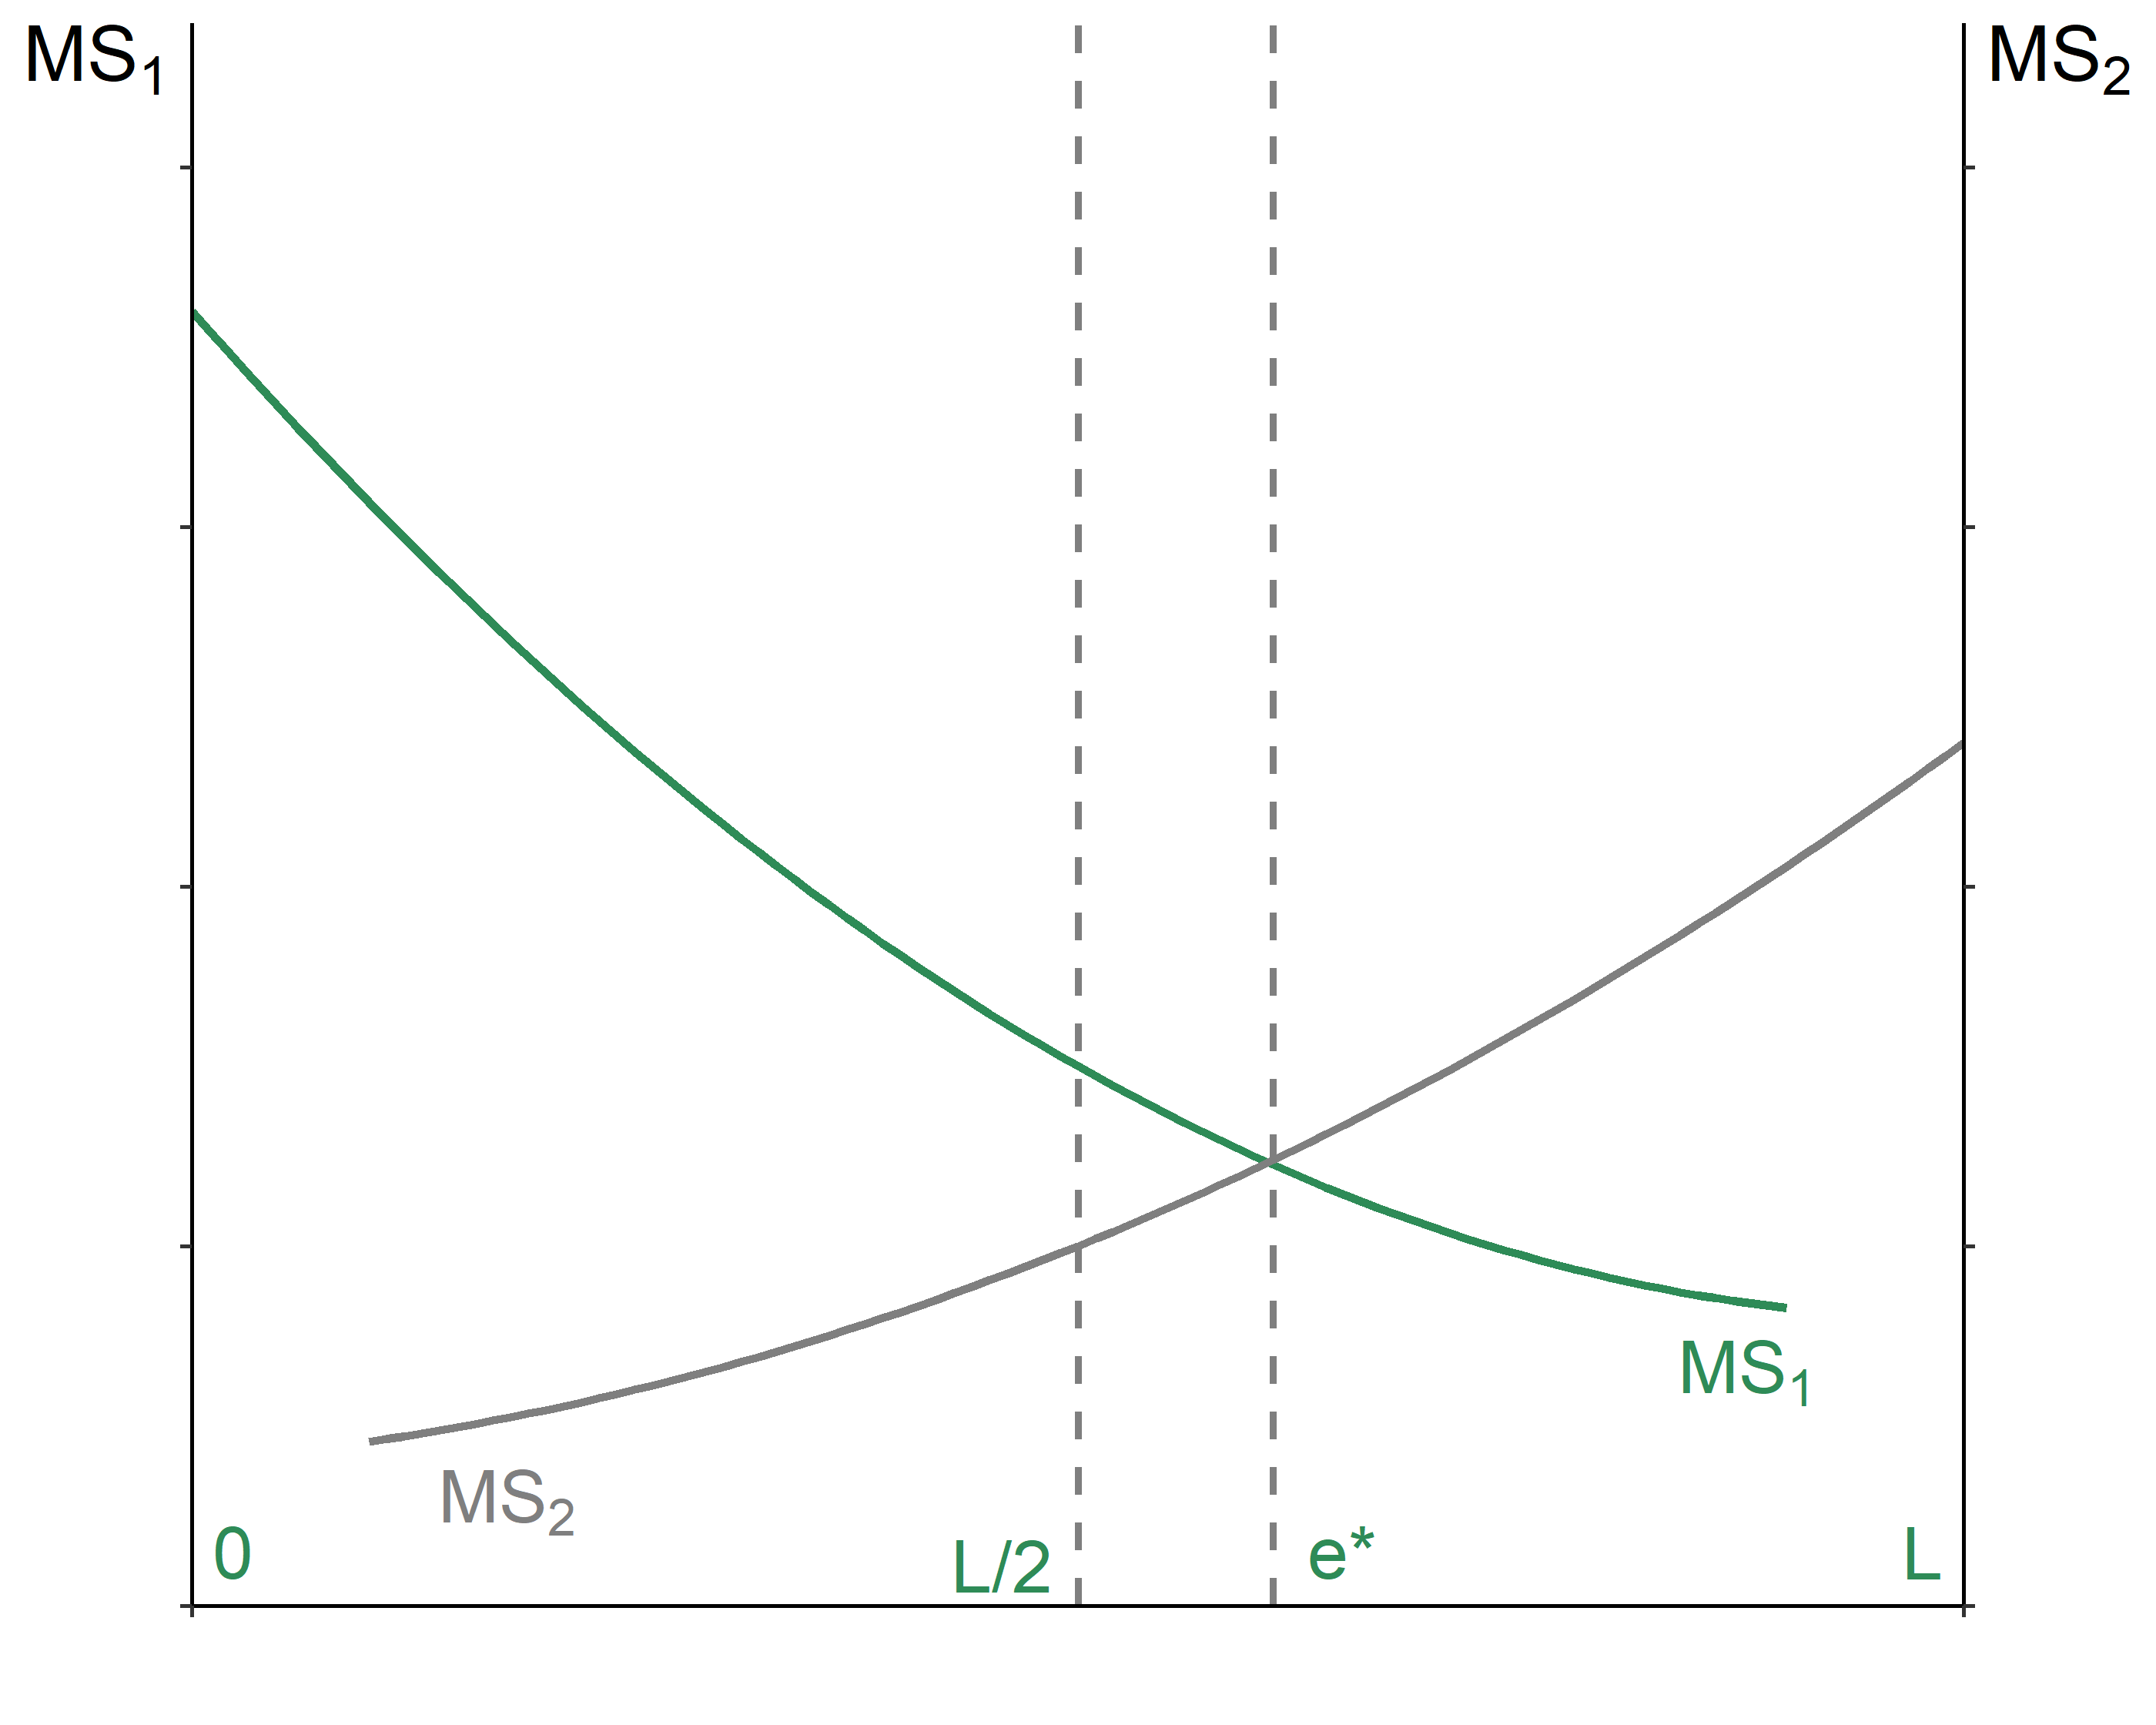
\includegraphics[width=0.9\linewidth]{envecon_files/figure-latex/permits-1} 

}

\caption{Marketable Permits}\label{fig:permits}
\end{figure}

The permits can be allocated for free, or being auctioned, with the revenue going to the government.

\hypertarget{emission-fees}{%
\section{Emission Fees}\label{emission-fees}}

Normally, consumer preferences for goods are communicated to producers through the price system. This system is ``broken'' in the case of environmental goods (or, rather, bads), because polluters' production function does not account for the damage caused by their emissions. A way to correct this is to establish an \emph{emission fee}---paid by a polluter to a regulatory entity for every unit of emission.

Consider a firm that produces some good, \(x\), and in the process emits pollution, \(e\). Let \(C(e)\), such that \(C'(e)<0\), denote the firm's costs for emission abatement. That is, the firm's costs (or efforts) to reduce pollution increase with the emission abatement. Further, let \(p\) be the emission fee, established by the regulator. So, the payment from the polluter to the regulator is \(pe\). Total emission--related costs for the firm, then, is given by the sum of the abatement costs and the payment associated with \(e\) units of emission: \[TC(e) = C(e)+pe.\] It then follows that at the optimum: \[p=-C'(e^*) \equiv MS(e^*),\] where \(MS(e)\) denotes the marginal savings from emitting one more unit of pollution.

The foregoing indicates that when faced with an emission fee, firms will abate pollution up to the point where the marginal savings (or marginal cost of abatement) is equal to the emission fee. Note that in this instance, the equimarginal principle automatically holds: each firm sets their marginal cost of abatement equal to the same emission fee.

\hypertarget{pigovian-taxes}{%
\section{Pigovian Taxes}\label{pigovian-taxes}}

A special kind of emission fee, which aims to restore Pareto optimality in the case of market failure, is known as the \emph{Pigovian tax}, after the English economist Arthur C. Pigou. In particular, a Pigovian tax is an emission fee that is exactly equal to the aggregate marginal damage caused by pollution when evaluated at the optimal level of pollution.

With multiple victims of pollution, the total damage is given by the vertical sum of individual damage functions: \[D(e) = \sum_{i=1}^{n}D_i(e),\] where \(n\) denotes the total number of people who are adversely affected from the pollution emitted by a firm. The efficient amount of pollution is the amount that minimizes the sum of costs and damages from pollution. So, at the optimum: \[MD(e^*) = MS(e^*).\] The emission fee associated with this optimal level of pollution is the Pigovian tax That is, the Pigovian tax is not just any emission fee; it is, indeed, the marginal savings from pollution at the optimal level of pollution.

\begin{figure}

{\centering 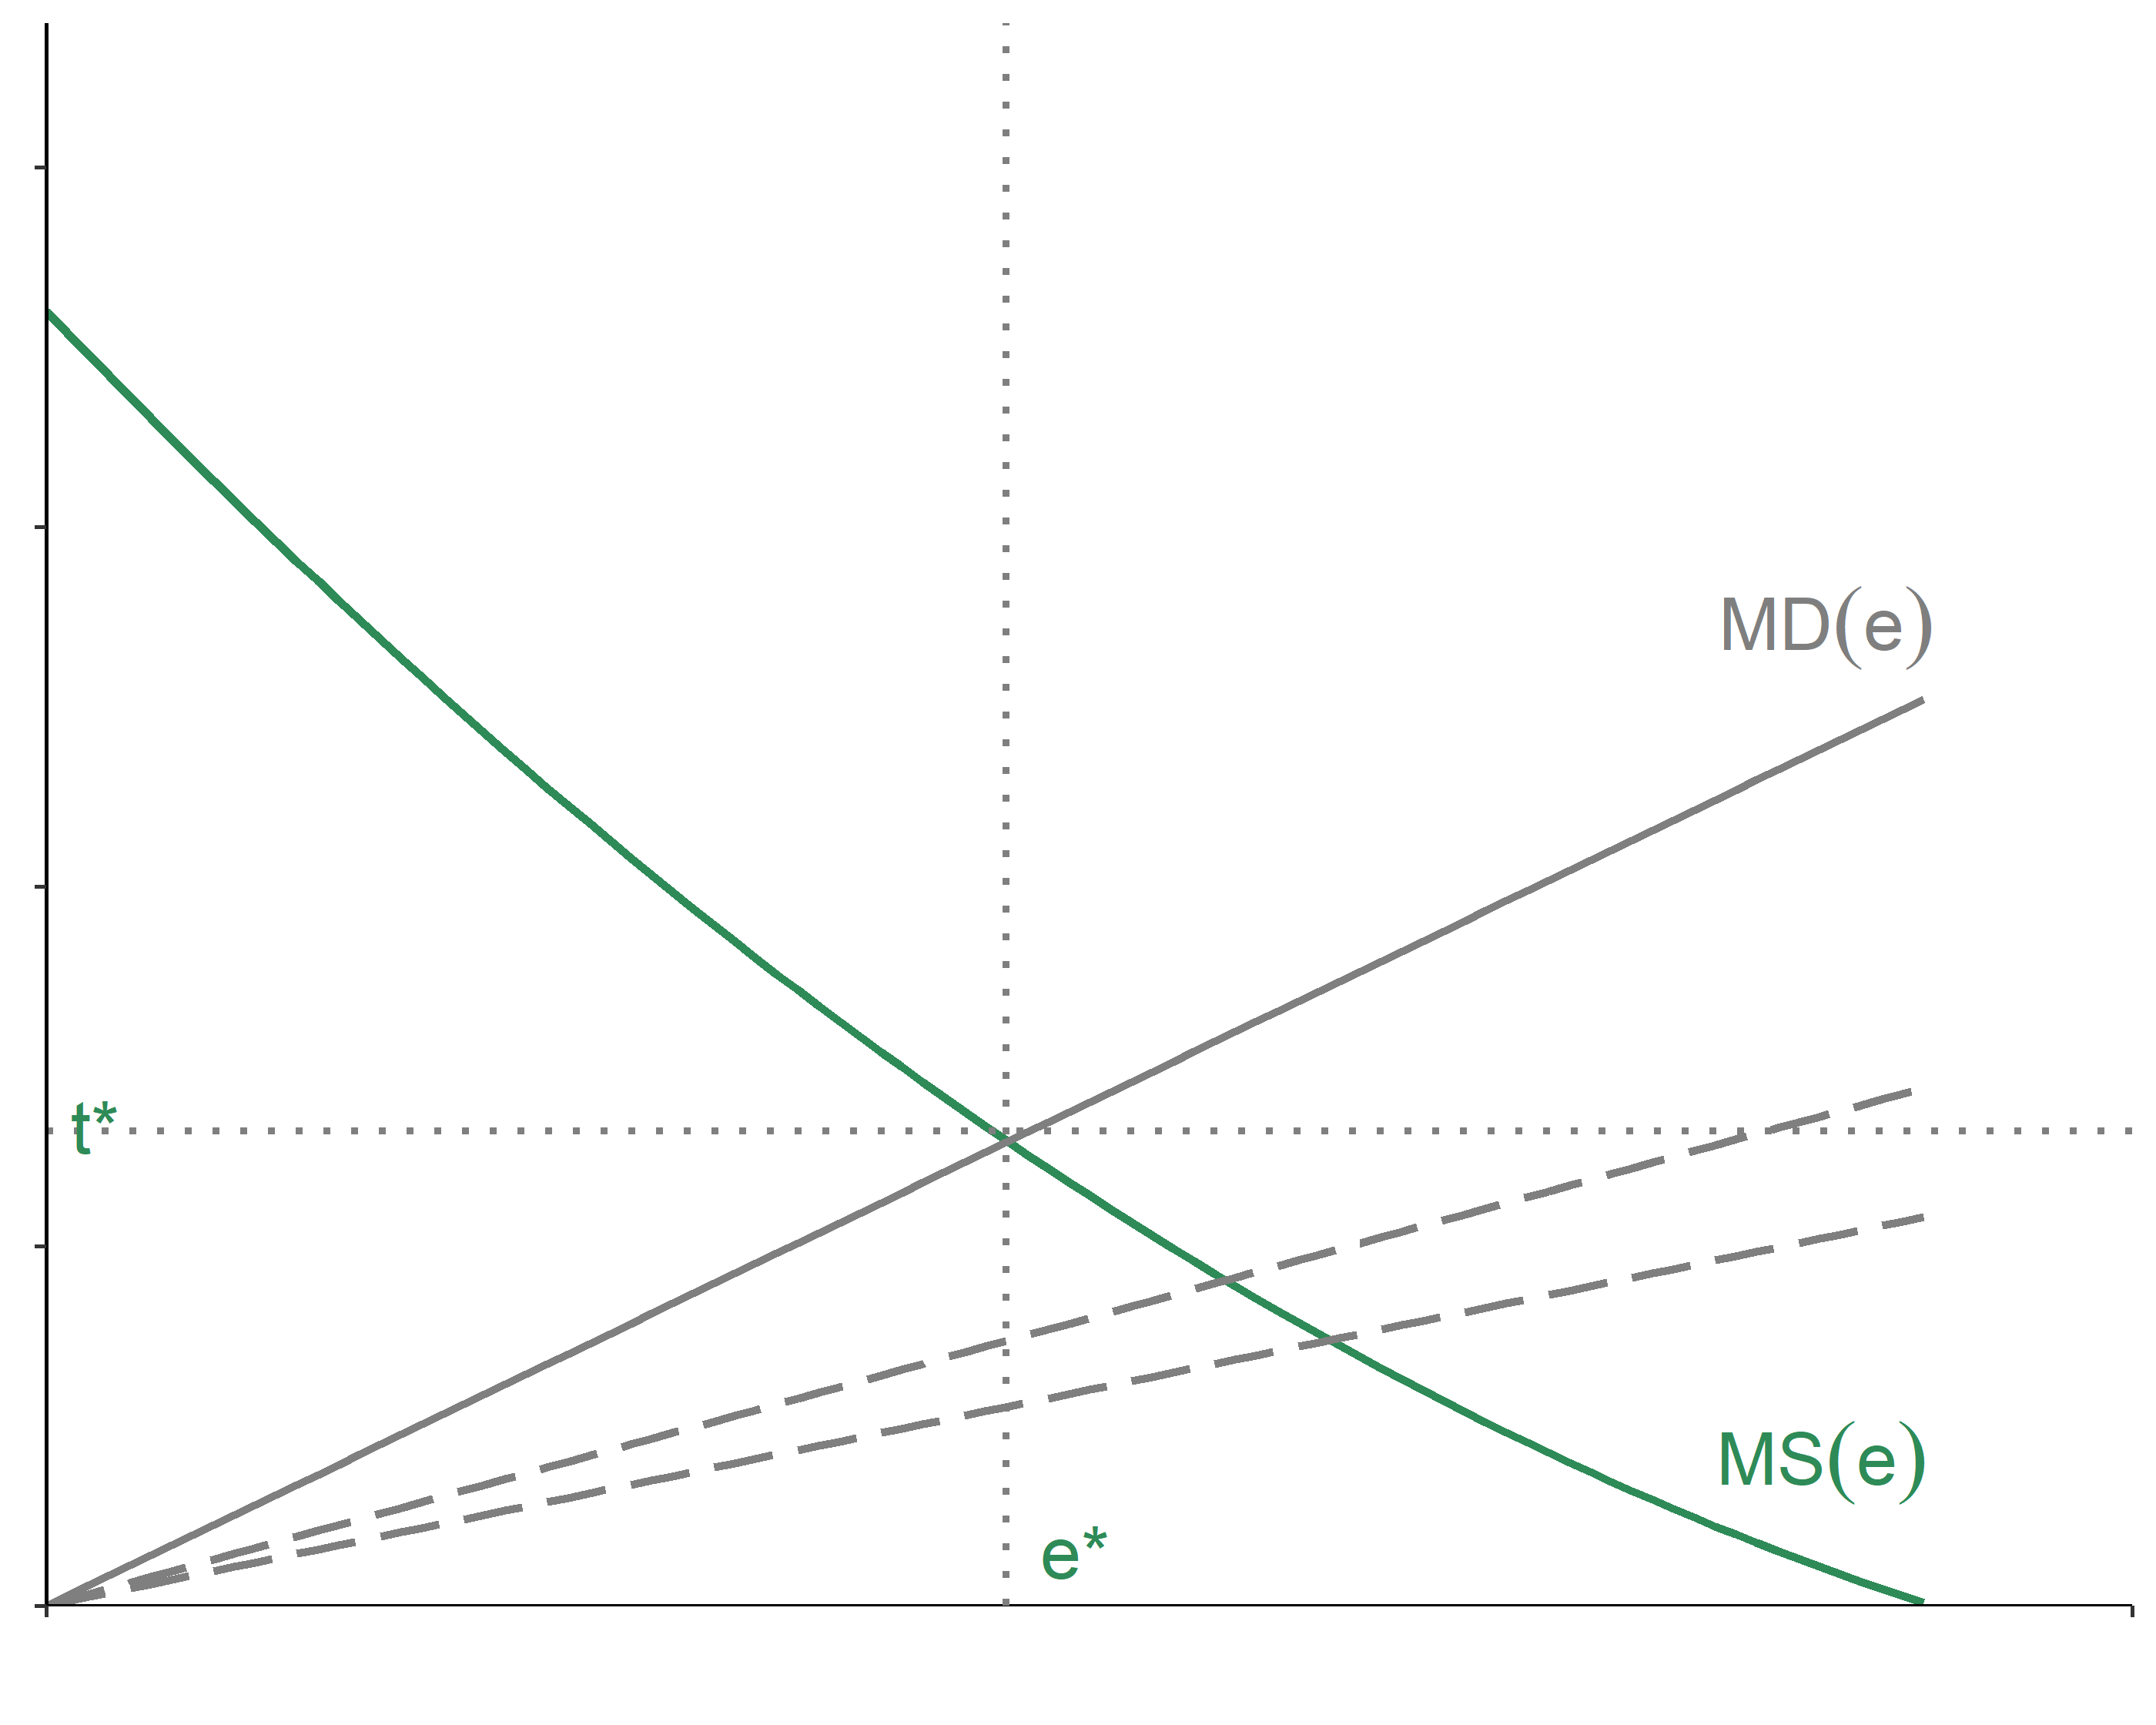
\includegraphics[width=0.9\linewidth]{envecon_files/figure-latex/pigou1-1} 

}

\caption{Optimal Pollution}\label{fig:pigou1}
\end{figure}

With multiple polluters, we typically assume that they are sharing the obligation of emission abatement in an efficient manner. The aggregate marginal savings is the horizontal sum of the individual marginal savings. Thus, for a given emission fee, the aggregate marginal savings tells us how much of pollution will be emitted in total, while the individual marginal savings tell us how much each firm will contribute to that total.

\begin{figure}

{\centering 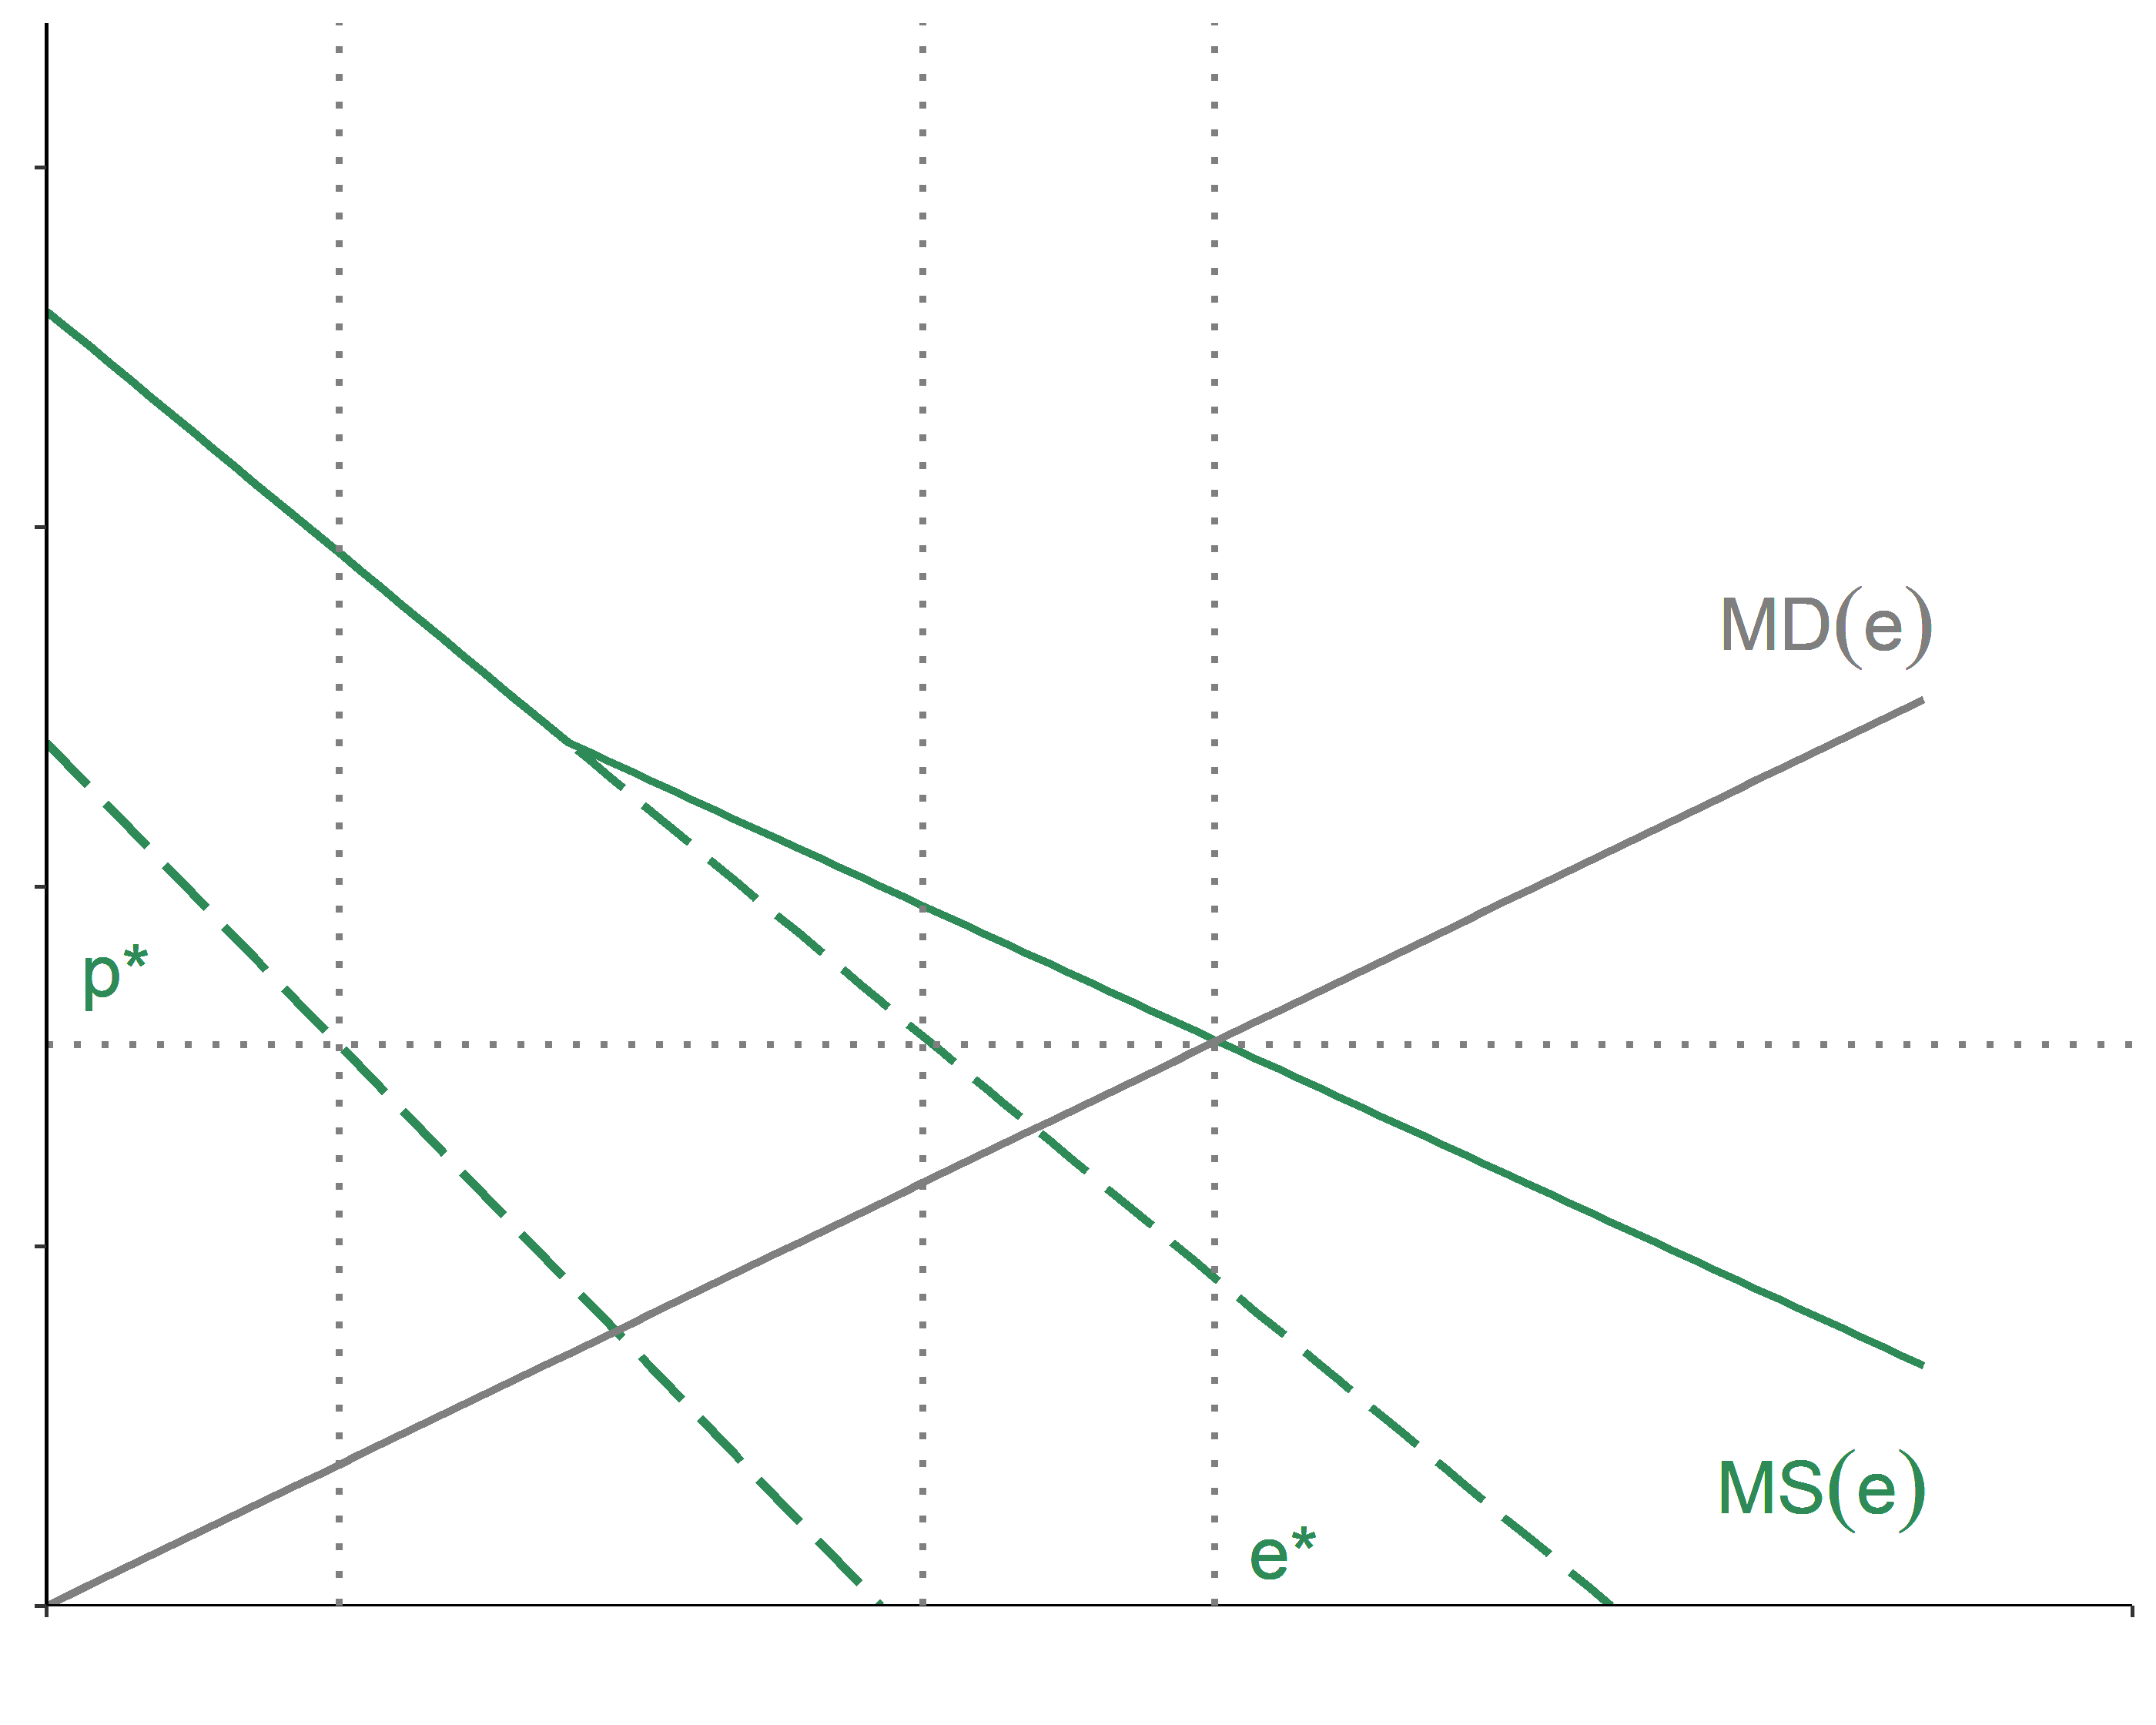
\includegraphics[width=0.9\linewidth]{envecon_files/figure-latex/pigou2-1} 

}

\caption{Optimal Pollution by Multiple Firms}\label{fig:pigou2}
\end{figure}

\hypertarget{regulation-with-information-asymmetry}{%
\chapter{Regulation with Information Asymmetry}\label{regulation-with-information-asymmetry}}

\hypertarget{imperfect-competition}{%
\section{Imperfect Competition}\label{imperfect-competition}}

When markets are not competitive, a host of efficiency problems arise, which, in turn, amplify the issues of environmental regulation. A case in point will be illustrated using two different scenarios: (i) a \emph{monopolist in the goods market} that is one of many polluters; and (ii) a competitive firm in the goods market that is the \emph{only polluter}.

\hypertarget{monopolist-in-production}{%
\subsection{Monopolist in Production}\label{monopolist-in-production}}

Consider a steel manufacturer that also emits pollution. There are many other polluters in the region, but only one steel manufacturer. In absence of regulation, the monopolist will produce where the marginal revenue and the unregulated marginal costs are equal.

The regulation will shift the marginal cost curve upward, and the firm will produce where the marginal revenue and the regulated marginal costs are equal. Turns out, the emission fee has made matters worse.

\begin{figure}

{\centering 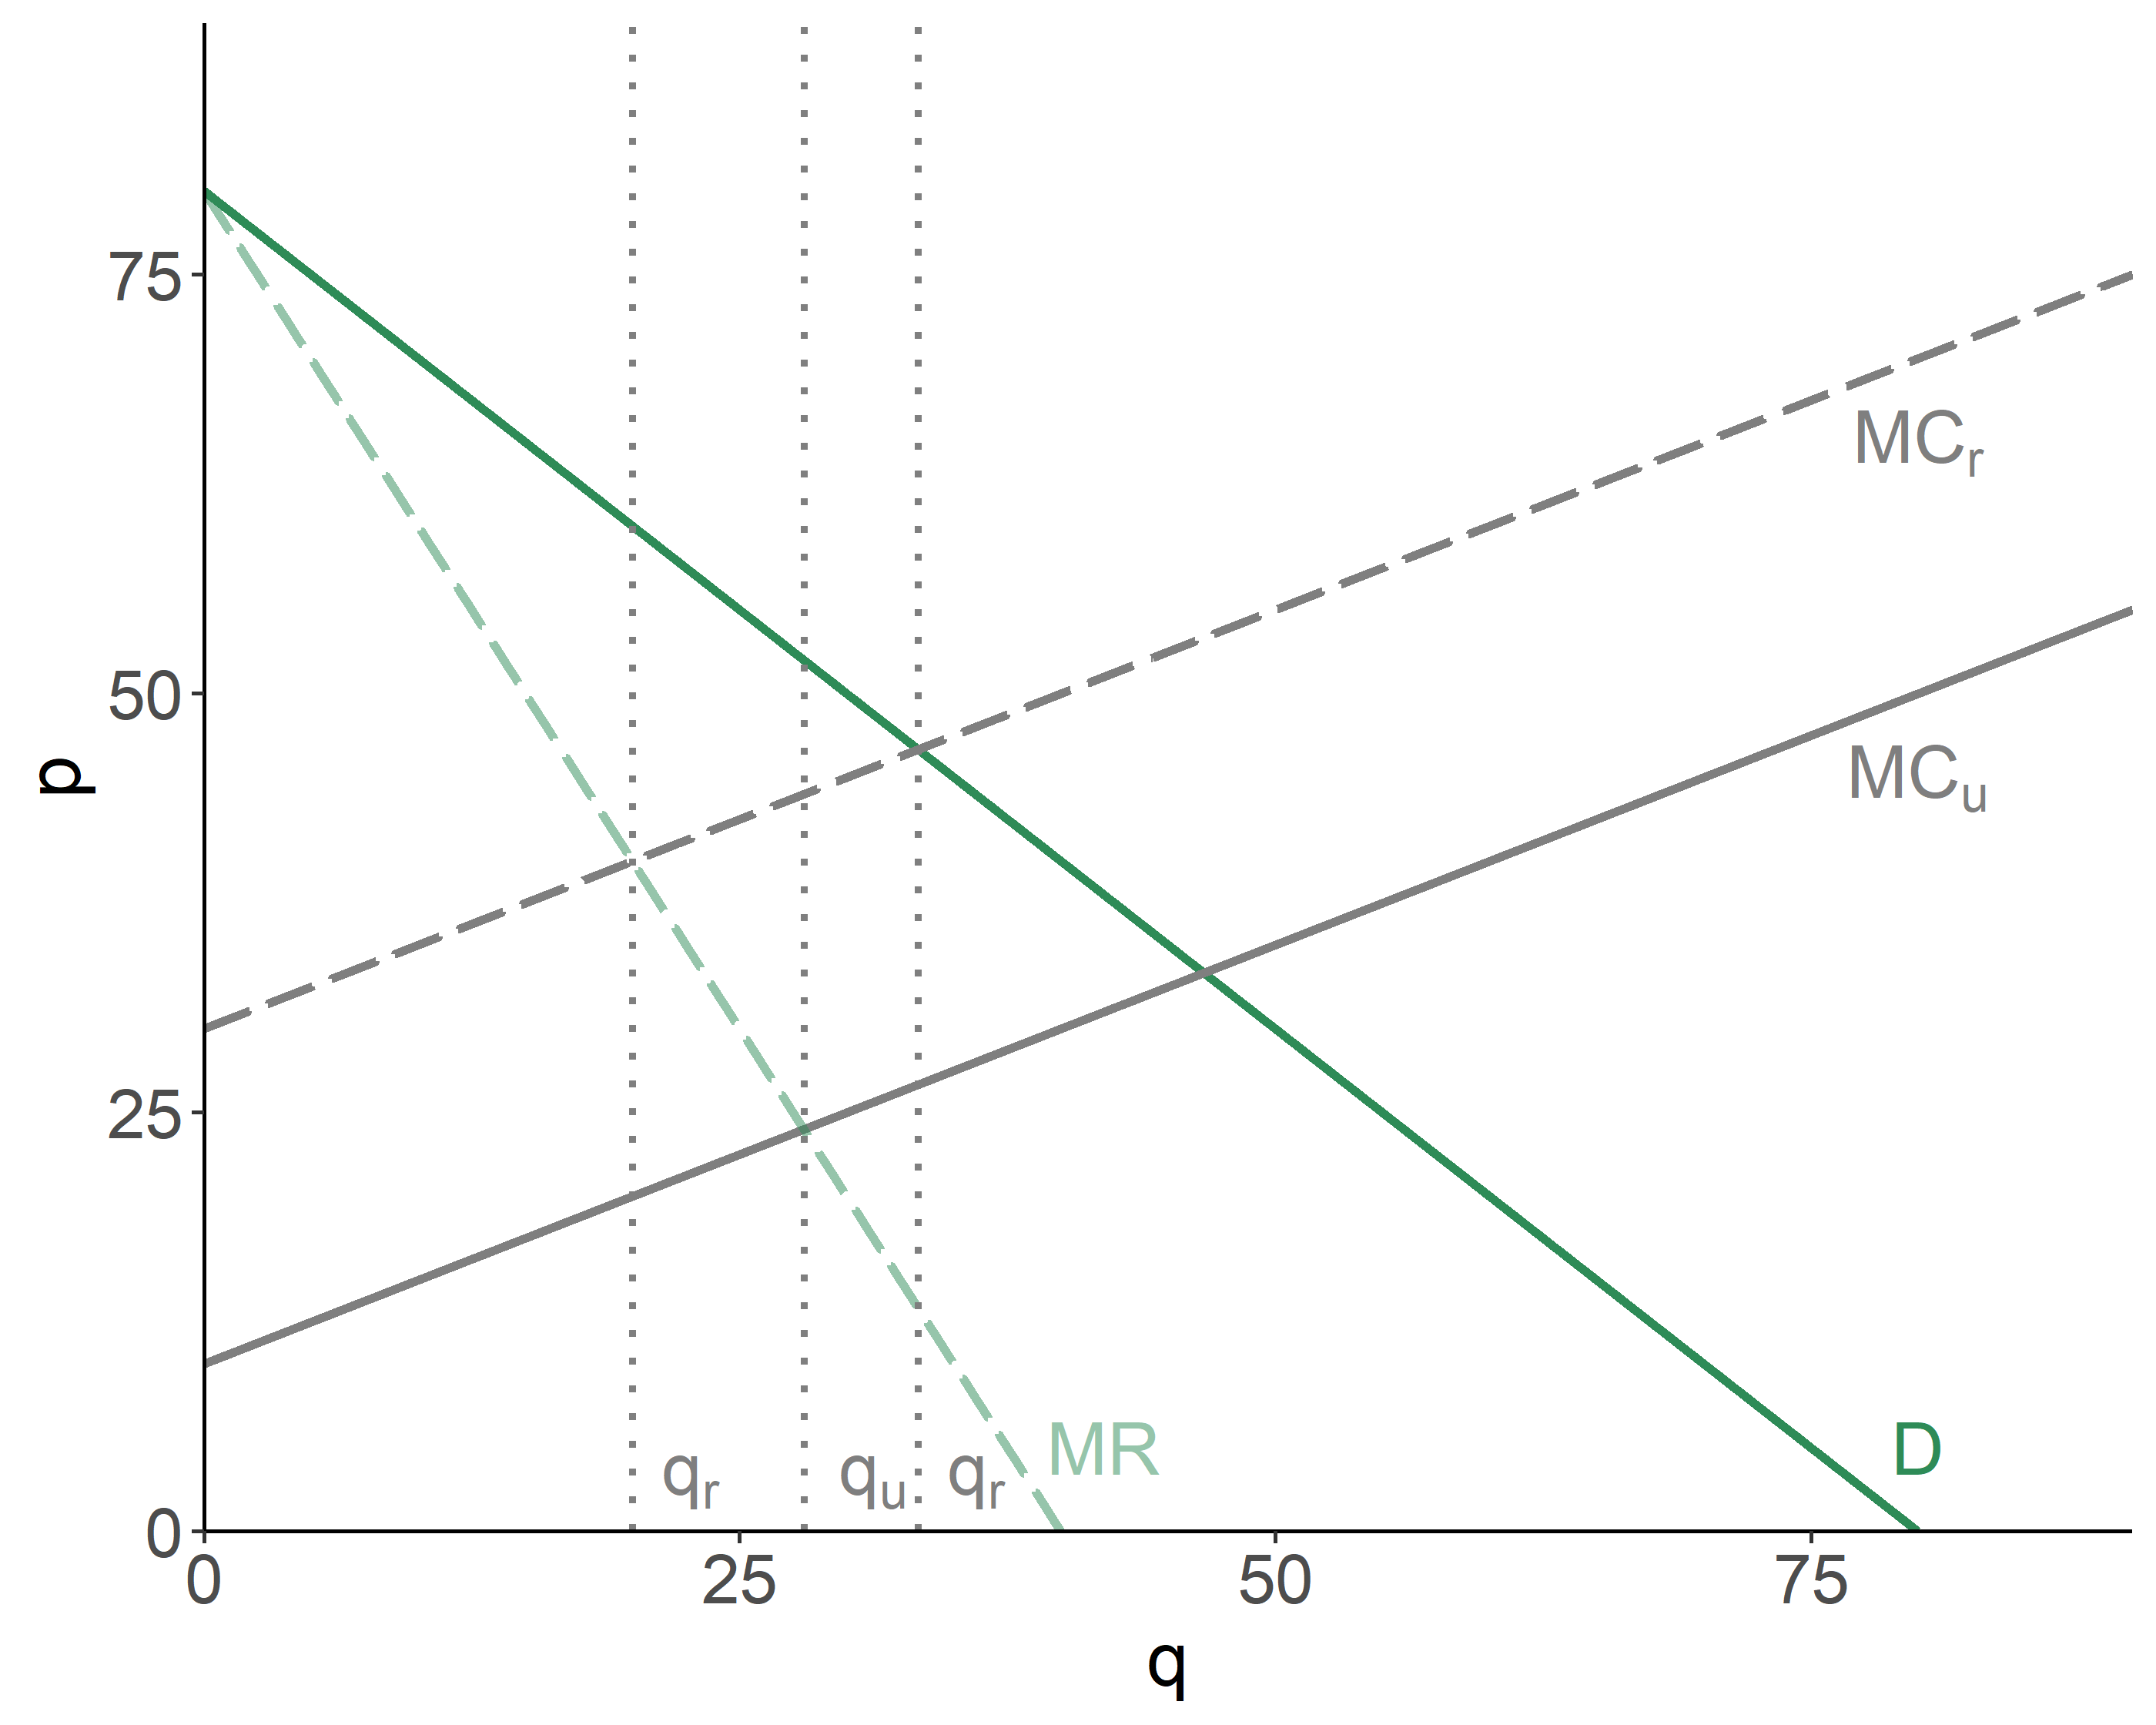
\includegraphics[width=0.9\linewidth]{envecon_files/figure-latex/monopoly1-1} 

}

\caption{Monopolist in Production and Pigovian Tax}\label{fig:monopoly1}
\end{figure}

The intuition behind this is simple: a monopolist has already lowered output below the competitive levels (which happen to be larger than the socially optimal levels). The imposition of the emission fee further restricts output, and in so doing may just overdo it.

\hypertarget{monopolist-in-emission}{%
\subsection{Monopolist in Emission}\label{monopolist-in-emission}}

Consider a firm, which is competitive in the goods market, but is a sole emitter of pollution in the region. That is, the firm is a monopolist in emission. The regulator imposes the emission tax, by setting it equal to the marginal damage of pollution. The firm, being able to observe the slope of the marginal damage function, will end up producing at the level that is below the efficient amount of pollution.

\begin{figure}

{\centering 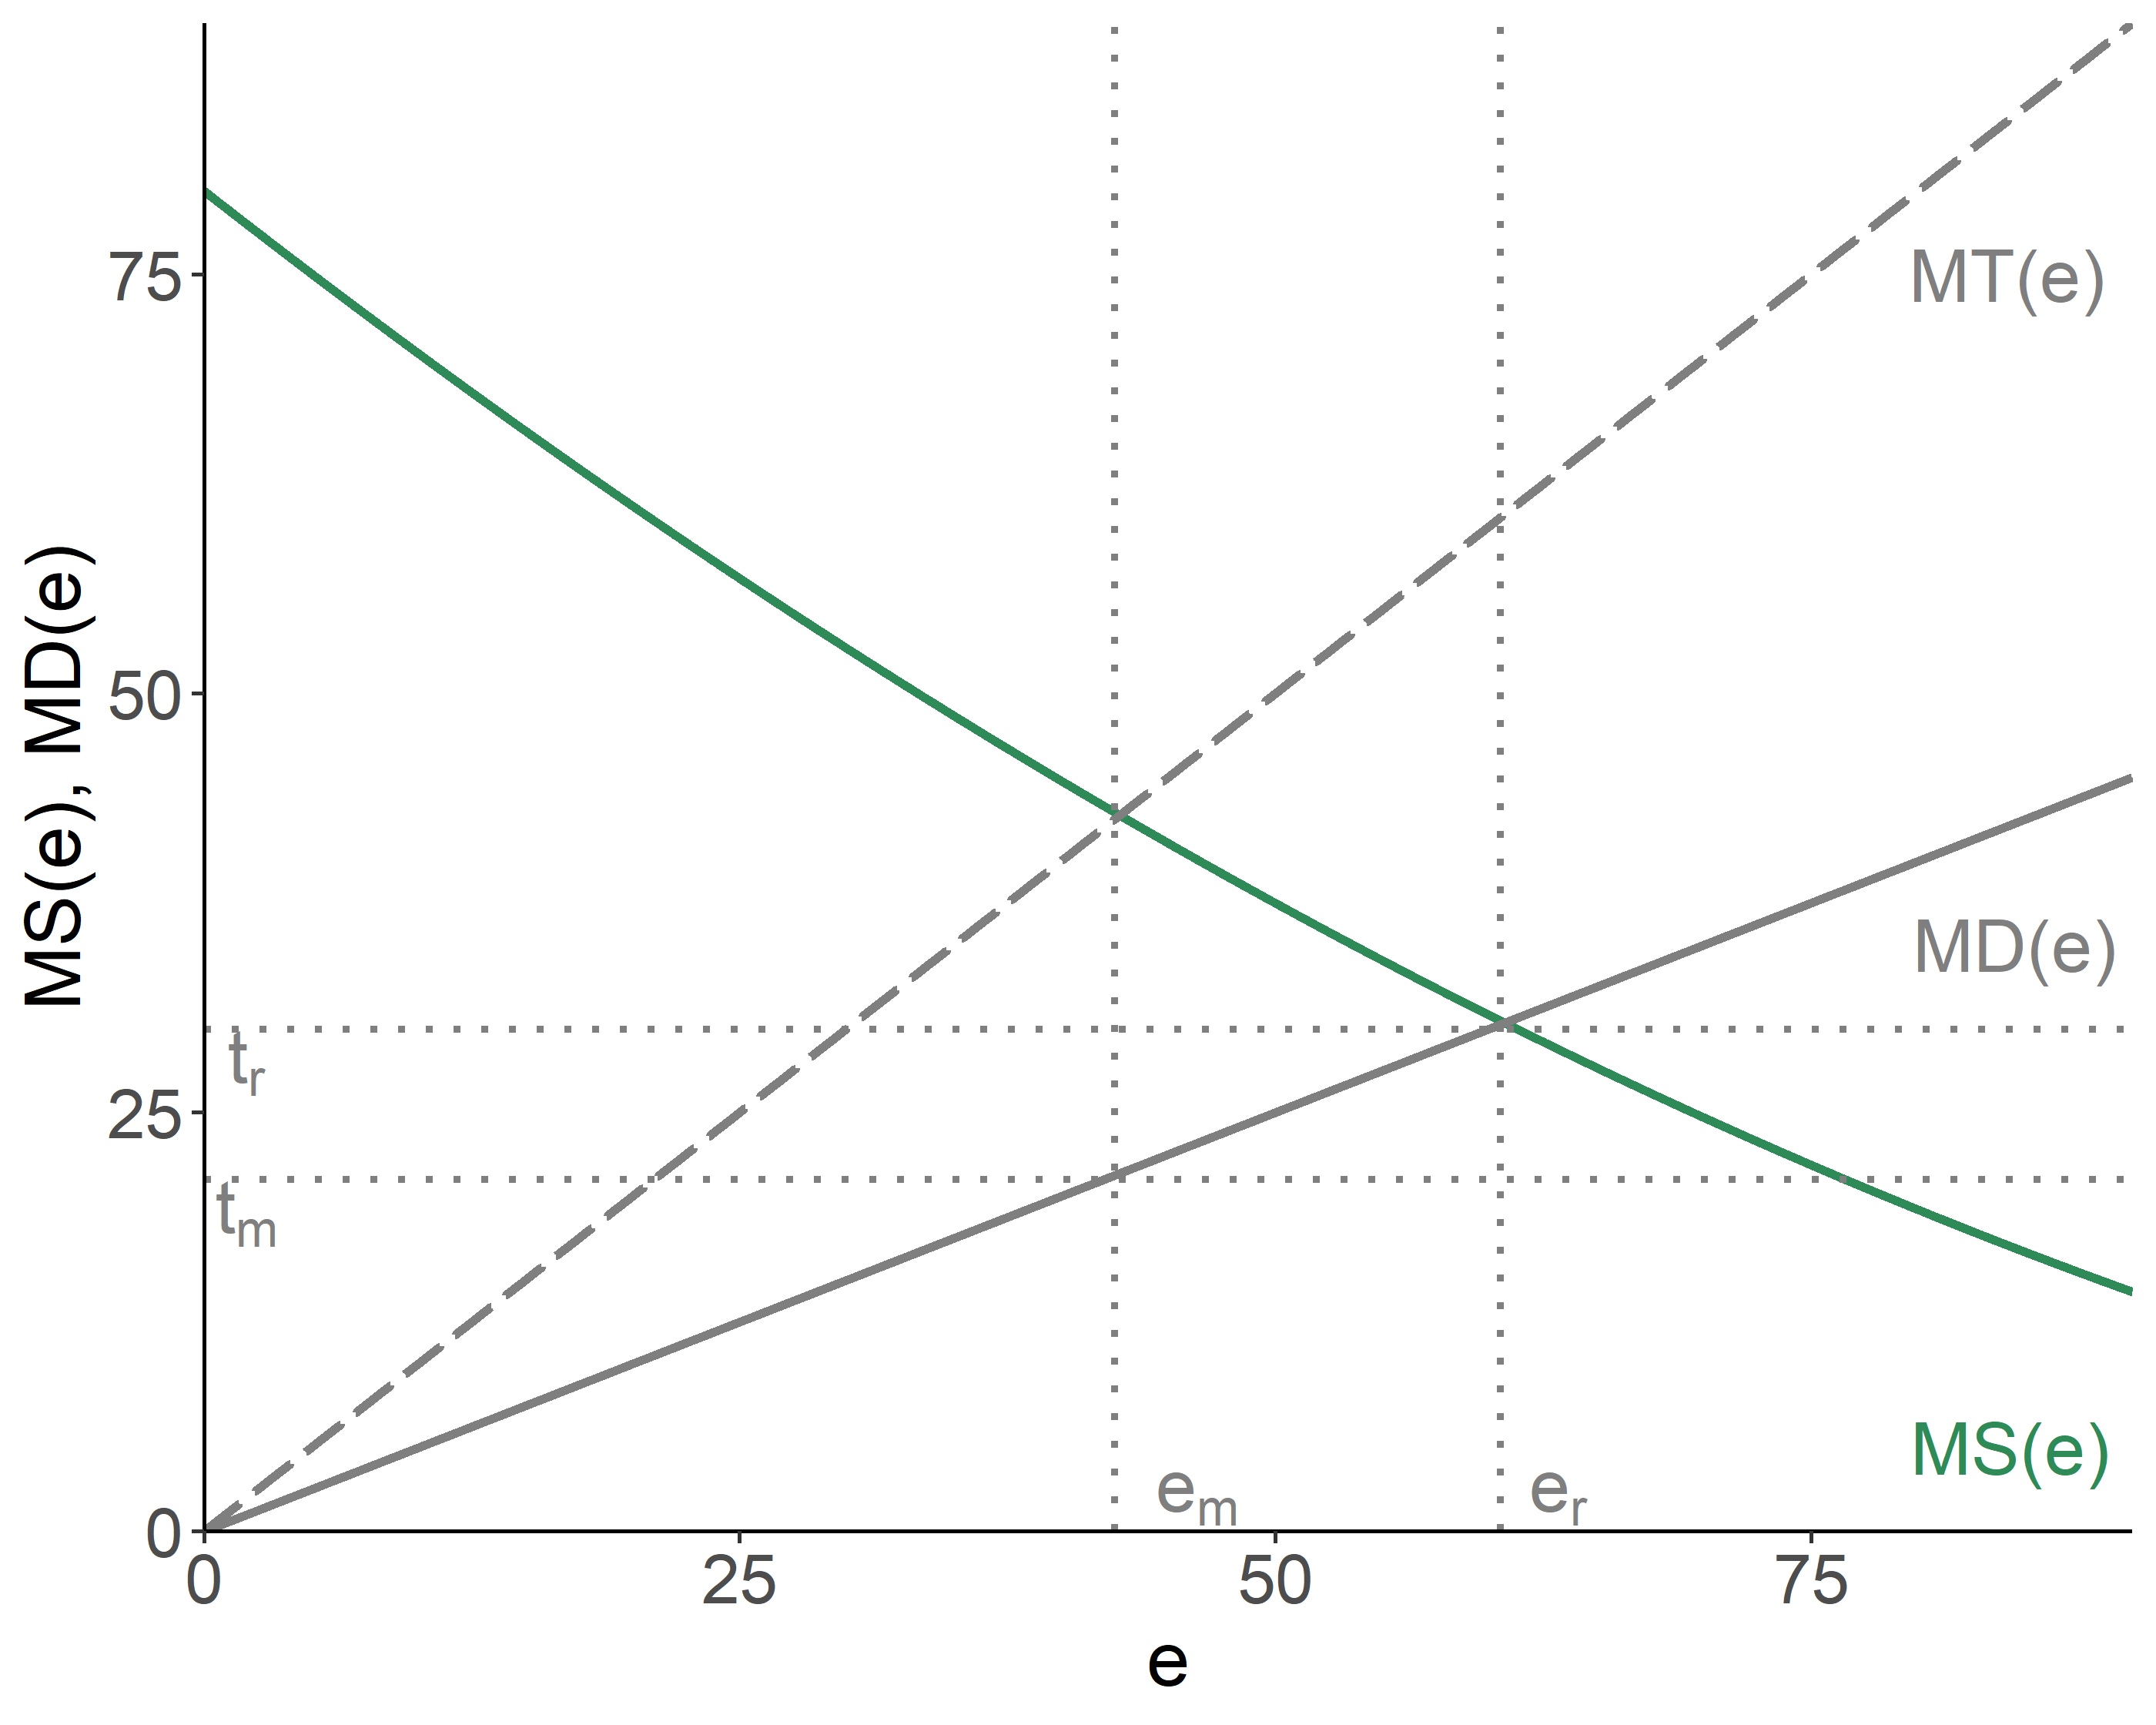
\includegraphics[width=0.9\linewidth]{envecon_files/figure-latex/monopoly2-1} 

}

\caption{Monopolist in Emission and Pigovian Tax}\label{fig:monopoly2}
\end{figure}

\hypertarget{limited-information-on-pollution-control}{%
\section{Limited Information on Pollution Control}\label{limited-information-on-pollution-control}}

Thus far we have assumed that a regulator knows exactly what pollution control costs are. A more realistic scenario, however, is that the regulator only possesses a limited fraction of the polluter's private information on control costs. In such case, a polluter may benefit from strategically misstating the costs. Questions to be addressed, then, are whether the information uncertainty related to control costs favors the use of emission permits vs.~fees as a more adequate means of regulation, and also whether there are benefits to an \emph{ex-ante} communication (information sharing) between a polluter and a regulator.

Suppose there are two types of polluters: those with high marginal savings from emission, \(MS_H(e)\), and those with low marginal savings from emission, \(MS_L(e)\). A single emission fee, \(\hat{\tau}\), thus will be either too low or too high, depending on the polluter type. Either way, there will be efficiency losses.

\begin{figure}

{\centering 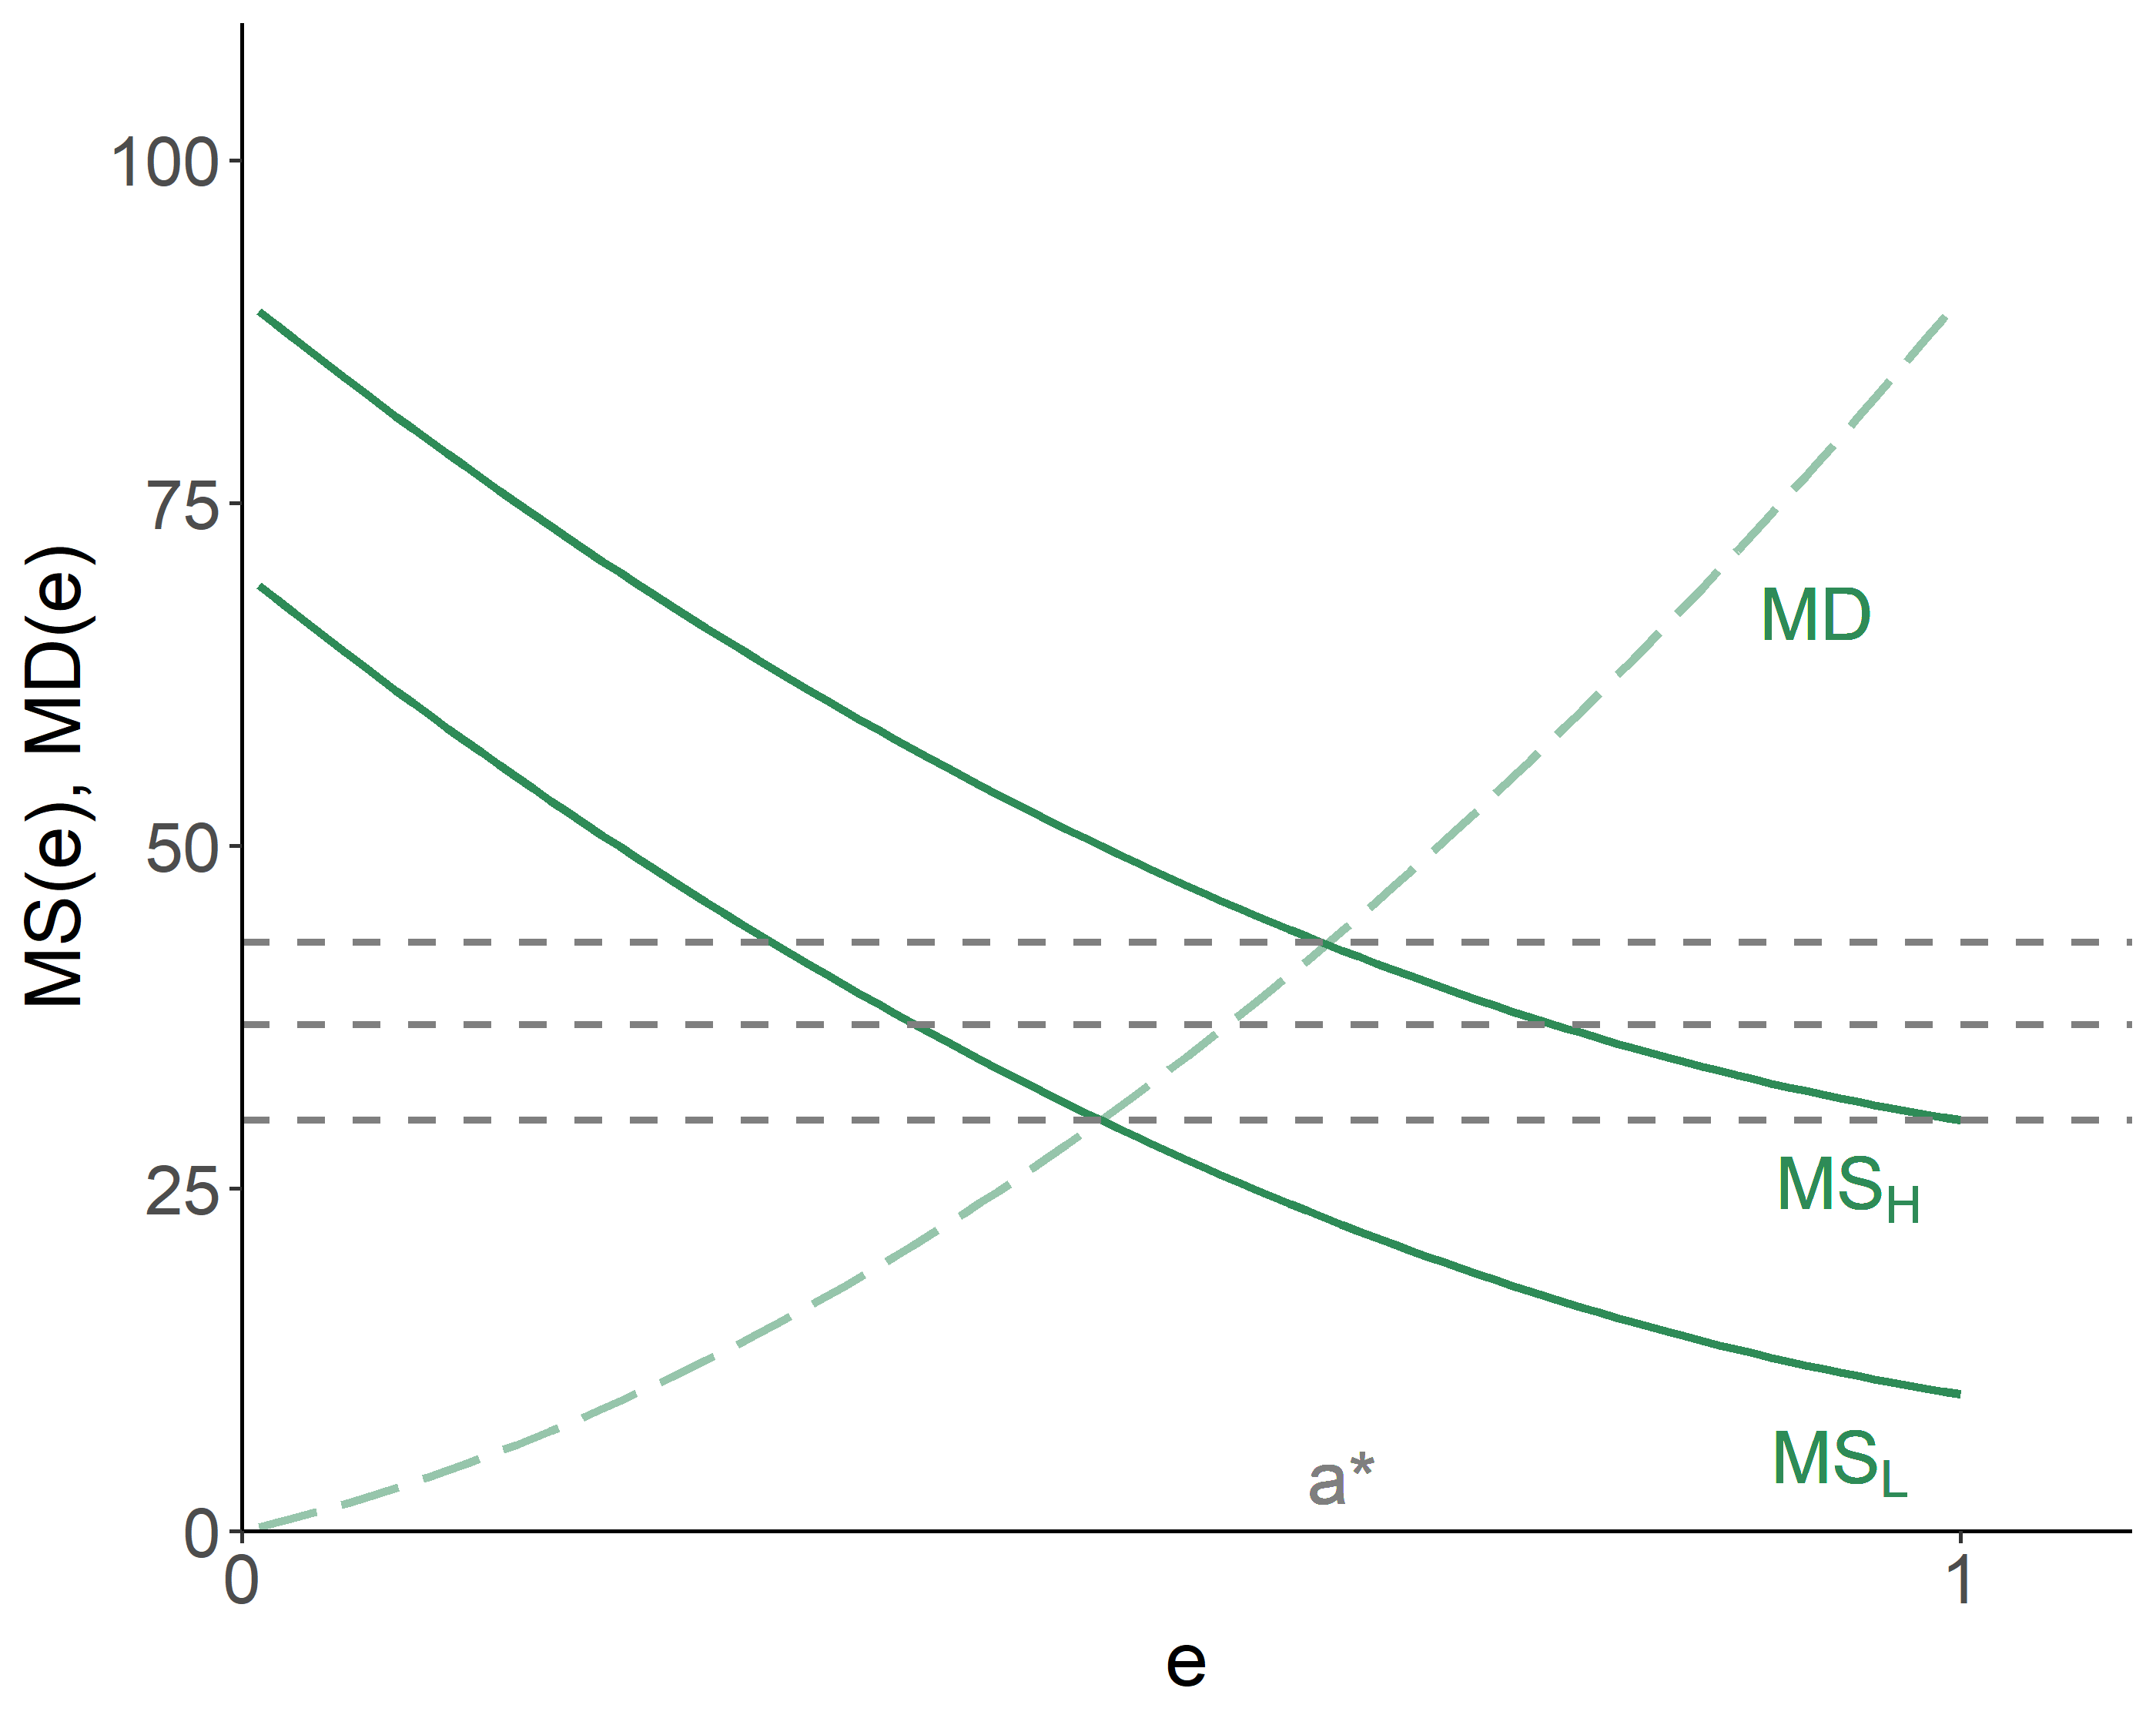
\includegraphics[width=0.9\linewidth]{envecon_files/figure-latex/uncertainty-1} 

}

\caption{Efficiency Losses}\label{fig:uncertainty}
\end{figure}

If a regulator knew exactly the type of a polluter, it would impose \(\tau_H^*\) on high-cost polluters, and \(\tau_L^*\) on low-cost polluters, and there would have been no efficiency losses. The issue exists, however, because polluters have incentives to misstate their actual type:

\begin{itemize}
\tightlist
\item
  if a regulator were to impose emission fees, a rational polluter would claim they are low-cost, regardless of their actual type;
\item
  if a regulator were to introduce permits, a rational polluter would claim they are high-cost, regardless of their actual type.
\end{itemize}

One way to `correct' the aforementioned adverse selection issue is by introducing a reward system of some sort for telling the truth. Consider the case of quantity regulations. Suppose a regulator is willing to introduce a reward, \(R\), to motivate truth-telling. So, polluters who claim they are high-cost get paid \(R_H\), and polluters who claim they are low-cost get paid \(R_L\). In fact, we can set \(R_H=0\) (recall: polluters have an in incentive to claim they are high-cost).

Each type of firm will tell the truth as long as that is the optimal strategy after the award has been factored in. For a high-cost firm, this means: \[C_H(e_H) < C_H(e_L)-R_L,\] and for a low-cost firm, this means: \[C_L(e_L)-R_L < C_L(e_H).\] Putting the two together, we obtain: \[C_L(e_L) - C_L(e_H) < R_L < C_H(e_L) - C_H(e_H)\]

Rewards aside, the benefit of lying for a low-cost firm is given by the area under their marginal savings curve, \(MS_L(e)\), and between the low and high levels of emission (respectively denoted by \(e_L\) and \(e_H\)); the benefit of telling the truth for a high-cost firm is given by the area under their marginal savings curve, \(MS_H(e)\), and between the low and high levels of emission.

\hypertarget{permits-vs.-fees}{%
\section{Permits vs.~Fees}\label{permits-vs.-fees}}

In absence of information asymmetry we saw that a regulator can reach the same outcome, in terms of emission levels, either with emission fees or emission permits. Uncertainty over emission costs, however, may distort such equivalence.

Consider a regulator and a firm. The regulator is aware that the firm can be of the high-cost or the low-cost marginal savings type. But unknown to the regulator remains the exact type of the firm. The regulator can implement either of the two options of emission control---a fee or a permit. But which one of these two is preferred? Martin Weitzman addressed this question in 1974, which led to what is now known as the \emph{Weitzman's Theorem}: with uncertainty over emission control costs, emission permits are preferred when marginal damages are more steeply sloped than marginal savings associated with emissions; otherwise, emission fees are preferred.

The issue with emission fees or permits is that neither of the two types of regulations has a flexibility to enforce pollution control, when it is relatively cheap to do so, but be a little more lenient, otherwise. It is, however, possible to introduce a hybrid regulation, where the permit system is coupled with the fee/subsidy mechanism.

The regulatory scheme is such that the firm is told to emit \(e^*\). If it emits less, it will receive subsidy, \(\sigma\), for each unit of pollution under the limit, and if it emits more, it will pay fee, \(\tau\), for each unit of pollution over the limit.

With such mechanism in place, if the firm's actual marginal savings are low, they will choose to emit \(\hat{e}_L\) and collect subsidy. If, on the other hand, the firm's marginal savings are high, they will emit \(\hat{e}_H\), which is above the allowed limit, and just pay the penalty for the difference.

The hybrid regulation allows us to achieve complete efficiency when there are only two marginal savings schedules.

When there are more than two types of firms---which is a more likely scenario---the hybrid regulation will not facilitate complete efficiency, but it will still do better than a pure emission fee or a pure emission permit scheme.

\hypertarget{regulation-across-space}{%
\chapter{Regulation Across Space}\label{regulation-across-space}}

One of the crucial dimensions of pollution manifestation is space---the degree of exposure to pollution often highly depends on location of those exposed. This complicates the regulator's task to optimally control pollution emission.

\hypertarget{emission-and-ambient-concentration}{%
\section{Emission and Ambient Concentration}\label{emission-and-ambient-concentration}}

Suppose there are several sources of emission, \(e_i\), where \(i=1,\ldots,n\). Each of them, to some extent, impact the air quality at some site, \(v_s\). We can express this relationship as follows: \[v_s = \sum_{i=1}^{n}a_{is}e_i,\] where \(a_{is}\) is the \emph{transfer coefficient} that links the emission from a source \(i\) with the ambient concentration at a receptor's site \(s\). For example, \(a_{is}\) can be a function of distance between \(e_i\) and \(v_s\). The concept of the transfer coefficient is particularly useful when the linearity assumption is maintained in the relationship between emissions and pollution.

Recall, the efficient amount of pollution involves equating marginal damages with marginal savings of emission. But, the marginal damage is, actually, measured in terms of ambient pollution. The relationship between the marginal damage \emph{in terms of emission} from source \(i\), and the marginal damage \emph{in terms of ambient concentration} at a receptor's site (to keep things simple we shall assume a single receptor, and drop subscript \(s\) from here forward), can be given by: \[MD(e_i) = a_{i}MD(v),\;~~i=1,\ldots,n.\]

Recognize that for any source, \(i\), \(MS(e_i) = MD(e_i)\); substitute it into the above equation and divide through by \(a_{i}\) to obtain: \[MS(e_i)/a_{i} = MD(v),\;~~i=1,\ldots,n.\] As it follows, two conditions are necessary for efficiency: (i) normalized marginal savings must be equalized for all sources; and (ii) normalized marginal savings must be equal to the marginal damage.

\hypertarget{ambientdifferentiated-emission-fees}{%
\subsection{Ambient--Differentiated Emission Fees}\label{ambientdifferentiated-emission-fees}}

When emission fees are imposed, the firms will respond by minimizing their total costs associated with emission, resulting in: \[MS(e_i) = t_i,\;~\forall\;i.\] It then follow that: \[t_i = a_i MD(v)\] and, to hold the equimarginal principle, \[t_i/a_i = t_j/a_j,\;~~\forall\;i,j.\] That is, the emission fees levied on the firms must be equal, after normalizing by the transfer coefficients.

While the ambient-differentiated emission fees can achieve efficiency, sometimes it is too complicated to vary the emission fee across locations, perhaps due to uncertainty about the transfer coefficients, or perceived unfairness to differentiate fees across firms.

Consider a two-firm scenario, and suppose they have the same marginal savings, but the transfer coefficients vary, resulting in different marginal damage curves. If a regulator were to differentiate, it would set fees at \(t_1\) and \(t_2\), respectively yielding emissions of \(e_1\) and \(e_2\), and incurring no losses in efficiency.

\begin{figure}

{\centering 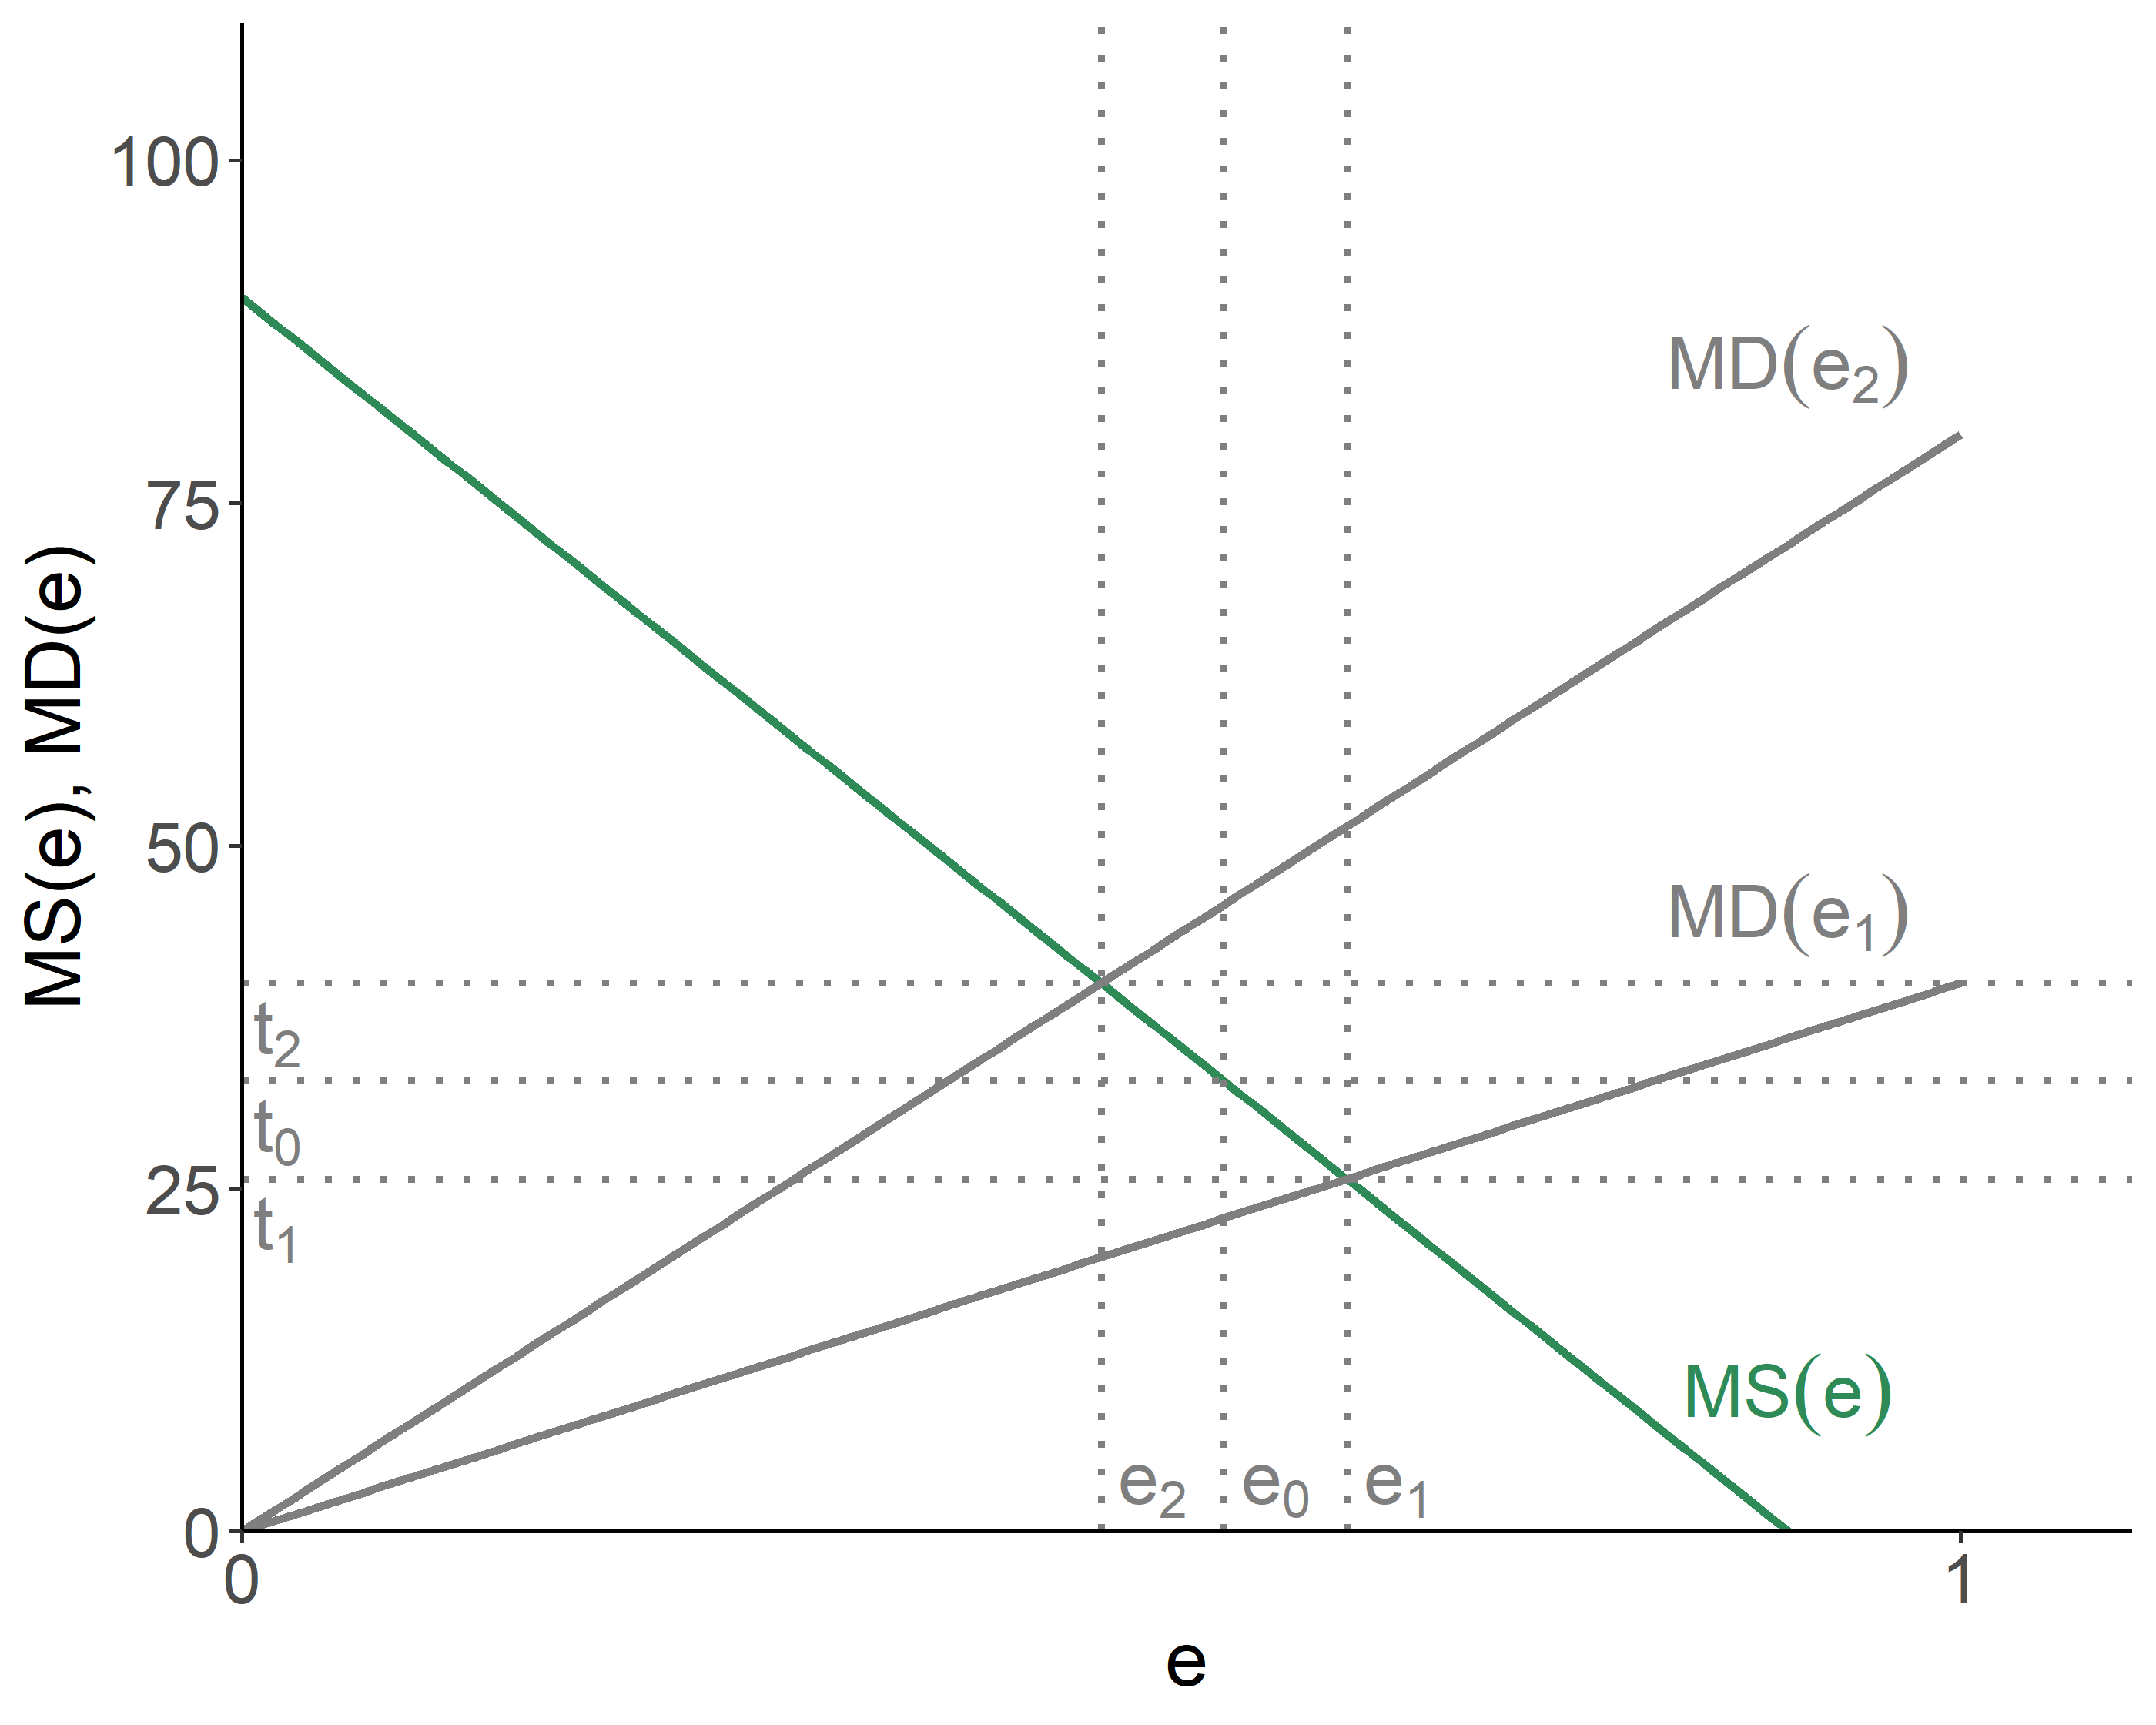
\includegraphics[width=0.9\linewidth]{envecon_files/figure-latex/inefficiency-1} 

}

\caption{Inefficiency of the Uniform Tax}\label{fig:inefficiency}
\end{figure}

But if a regulator were to use a uniform tax, \(t_0\), both firms would emit the same amount of pollution, \(e_0\), which will result in efficiency losses depicted by: (1) an area between \(e_0\) and \(e_1\), below \(MS(e)\) and above \(MD(e_1)\); and (2) an area between \(e_0\) and \(e_2\), above \(MS(e)\) and below \(MD(e_2)\). If such uniform fee were to be the regulator's only option, the `optimal' tax would be the one that minimizes the said efficiency losses.

\hypertarget{marketable-ambient-permits}{%
\section{Marketable Ambient Permits}\label{marketable-ambient-permits}}

An emission permit system---that take into account the effect of ambient concentration in the affected locations---is somewhat more complicated, but (in theory) can work just as well as ambient-differentiated emission fees.

Consider a case of two firms and one receptor. If a regulator (randomly) assigns a total of \(L=L_1+L_2\) permits to these firms, the questions to be answered will be: (i) what will the price of permits be? and (ii) how much will each firm emit?

Let \(r\) denote the price of permits, and \(l_1\) and \(l_2\) denote the number of permits eventually held by the firms. Note that: \(l_1=a_1 e_1\) and \(l_2=a_2 e_2\), resulting in \(a_1 e_1 + a_2 e_2 =L\). A firm's total costs are: \[TC(e_i) = C(e_i)+(a_i e_i - L_i)r,\;~~i=1,2.\] Cost minimization (with respect to \(e_i\)) results in the optimality conditions: \[MS(e_i)/a_i = r,\;~~i=1,2.\] We thus can solve the three equations for three unknowns (\(e_1\), \(e_2\), and \(r\)).

\hypertarget{zonal-instruments}{%
\section{Zonal Instruments}\label{zonal-instruments}}

There can be a middle ground between completely undifferentiated emission fees or permits (i.e., where space is ignored) and ambient fees or permits.

In the case of fees, a region is divided into zones. Within each zone, the same emission fee applies, but fees may vary across the zones. The advantage of such zonal system is more flexibility, resulting in efficiency gains (over the undifferentiated system). The disadvantages are those inherited from the ambient fee system (note that as zones become small and numerous, a zonal fee system, in essence, becomes an ambient fee system).

As for permits, within a zone, they are traded on a 1-for-1 basis. Across the zones, however, a permit trading system applies different transfer coefficients for different zones. There are efficiency gains from a zonal system, accompanied by disadvantages due to complexity associated with the ambient permit system.

\hypertarget{regulation-over-time}{%
\chapter{Regulation Over Time}\label{regulation-over-time}}

\hypertarget{climate-change-and-adaptation}{%
\chapter{Climate Change and Adaptation}\label{climate-change-and-adaptation}}

\hypertarget{references}{%
\chapter*{References}\label{references}}
\addcontentsline{toc}{chapter}{References}

\hypertarget{refs}{}
\leavevmode\hypertarget{ref-adamowicz1998}{}%
Adamowicz, Wiktor, Peter Boxall, Michael Williams, and Jordan Louviere. 1998. ``Stated Preference Approaches for Measuring Passive Use Values: Choice Experiments and Contingent Valuation.'' \emph{American Journal of Agricultural Economics} 80 (1): 64--75.

\leavevmode\hypertarget{ref-isaksen2019}{}%
Isaksen, Elisabeth Thuestad, and Andries Richter. 2019. ``Tragedy, Property Rights, and the Commons: Investigating the Causal Relationship From Institutions to Ecosystem Collapse.'' \emph{Journal of the Association of Environmental and Resource Economists} 6 (4): 741--81.

\leavevmode\hypertarget{ref-keohane2016}{}%
Keohane, Mr Nathaniel O, and Sheila M Olmstead. 2016. \emph{Markets and the Environment}. Island Press.

\leavevmode\hypertarget{ref-keohane2009}{}%
Keohane, Nathaniel O. 2009. ``Cap and Trade, Rehabilitated: Using Tradable Permits to Control US Greenhouse Gases.'' \emph{Review of Environmental Economics and Policy} 3 (1): 42--62.

\leavevmode\hypertarget{ref-kolstad2010}{}%
Kolstad, Charles D. 2010. \emph{Environmental Economics}. 2nd ed. Oxford University Press.

\end{document}
